% main.tex - Master file for Python for Scientists
% ============================================================================
% Compile with: pdflatex main.tex (run twice for TOC)
% Or use: latexmk -pdf main.tex
% ============================================================================

\input{preamble}

% ============================================================================
% DOCUMENT METADATA
% ============================================================================
\title{Python and Computational Thinking:\\[0.5em]
       \Large A Crash Course for Scientists}
\author{Frithjof Herb}
\date{\today}

% ============================================================================
% BEGIN DOCUMENT
% ============================================================================
\begin{document}

% ----------------------------------------------------------------------------
% FRONT MATTER
% ----------------------------------------------------------------------------
\frontmatter

% Title page
\input{frontmatter/titlepage}

% Table of contents
\tableofcontents

% Preface and how to use
\input{frontmatter/preface}
% how_to_use.tex - Guide to reading and using this book
% ============================================================================

\chapter*{How to Use This Book}
\addcontentsline{toc}{chapter}{How to Use This Book}

\section*{Read in Order (At First)}

The chapters build on each other. Chapter 2 assumes you completed Chapter 1. Skipping ahead usually leads to confusion and backtracking. Once you've worked through the whole book, it becomes a useful reference for jumping to specific topics. But for first-time learners: start at the beginning.

\section*{Special Boxes}

Throughout the book, you'll find colored boxes that highlight different types of information:

\begin{warning}
\textbf{Warnings} alert you to common mistakes and pitfalls. Pay attention to these---they'll save you debugging time.
\end{warning}

\begin{tip}
\textbf{Tips} offer shortcuts, best practices, or alternative approaches that experienced programmers use.
\end{tip}

\begin{note}
\textbf{Notes} provide additional context or clarification that might help your understanding but isn't strictly necessary.
\end{note}

\begin{osbox}
\textbf{OS Differences} explain when something works differently on Windows, macOS, or Linux. Most of Python is identical across systems, but installation and file paths sometimes differ.
\end{osbox}

\begin{labexample}
\textbf{Lab Examples} connect programming concepts to real scientific scenarios. These show how you might actually use what you're learning in your research.
\end{labexample}

\begin{ponder}
\textbf{Things to Ponder} are reflection questions at the end of sections. You don't need to answer them in writing, but thinking about them helps solidify concepts.
\end{ponder}

\section*{Code Examples}

Code appears in monospace font with syntax highlighting:

\begin{lstlisting}
# This is Python code
temperature = 298.15  # Kelvin
print(f"Temperature: {temperature} K")
\end{lstlisting}

When we show interactive Python sessions (the REPL), you'll see \py{>>>} prompts:

\begin{lstlisting}
>>> 2 + 2
4
>>> "hello".upper()
'HELLO'
\end{lstlisting}

Lines starting with \py{>>>} are what you type. Lines without are Python's output.

\section*{Typing vs. Copying}

Type the code examples yourself. Yes, it's slower than copy-pasting. That's the point. Typing forces you to read every character, notice the syntax, and build muscle memory. It also means you'll make typos, see error messages, and learn to fix them---all valuable skills.

\section*{Data Files}

Some examples use data files (CSV files, text files with measurements, etc.). These are available in the \filepath{data/} folder that accompanies this book. When an example references a file like \filepath{titration\_data.csv}, you'll find it there.

\section*{Getting Unstuck}

When something doesn't work:

\begin{enumerate}
    \item Read the error message carefully. Python tells you what's wrong.
    \item Check for typos. Case matters. Indentation matters. Quotes must match.
    \item Re-read the relevant section. Something may have not registered the first time.
    \item Search online. Copy-paste the error message into a search engine. Someone else has had the same problem.
    \item Take a break. Fresh eyes find bugs faster.
\end{enumerate}

Debugging is part of programming. Getting stuck doesn't mean you're bad at this---it means you're learning.


% ----------------------------------------------------------------------------
% MAIN MATTER
% ----------------------------------------------------------------------------
\mainmatter

% Part I: Getting Started
\part{Getting Started}
\input{chapters/chap00_setup}

% Part II: Python Fundamentals
\part{Python Fundamentals}
\input{chapters/chap01_basics}
% chap02_containers.tex - Lists, dicts, sets, and tuples
% ============================================================================

\chapter{Container Types}
\label{chap:containers}

So far, each variable holds one value. But scientific data comes in groups: a series of measurements, a collection of samples, a table of properties. Python's container types hold multiple values in a single variable. This chapter covers the four main ones: lists, tuples, dictionaries, and sets.

% ----------------------------------------------------------------------------
\section{Lists}
\label{sec:lists}

A list is an ordered collection of items. Create one with square brackets:

\begin{lstlisting}
>>> temperatures = [20.1, 21.3, 19.8, 22.0, 20.5]
>>> temperatures
[20.1, 21.3, 19.8, 22.0, 20.5]
>>> elements = ["H", "He", "Li", "Be", "B"]
>>> elements
['H', 'He', 'Li', 'Be', 'B']
\end{lstlisting}

Lists can contain any type of data, and items don't have to be the same type (though they usually are):

\begin{lstlisting}
>>> mixed = [1, "hello", 3.14, True]
>>> mixed
[1, 'hello', 3.14, True]
\end{lstlisting}

\subsection{Indexing}

Access individual items by position using square brackets. The position number is called the \emph{index}. Python uses zero-based indexing---the first item is at index 0, not index 1. This is a common convention in programming (though not universal), so get used to it:

\begin{lstlisting}
>>> elements = ["H", "He", "Li", "Be", "B"]
>>> elements[0]       # first item
'H'
>>> elements[1]       # second item
'He'
>>> elements[4]       # fifth item (last in this list)
'B'
>>> elements[-1]      # last item (negative indexing)
'B'
>>> elements[-2]      # second to last
'Be'
\end{lstlisting}

\begin{warning}
Accessing an index that doesn't exist causes an error:
\begin{lstlisting}
>>> elements[10]
IndexError: list index out of range
\end{lstlisting}
Always check your list length if you're unsure.
\end{warning}

\subsection{Slicing}

Extract a sublist using slice notation \py{[start:stop]}:

\begin{lstlisting}
>>> numbers = [0, 1, 2, 3, 4, 5, 6, 7, 8, 9]
>>> numbers[2:5]      # items from index 2 up to (not including) 5
[2, 3, 4]
>>> numbers[:4]       # from beginning to index 4
[0, 1, 2, 3]
>>> numbers[6:]       # from index 6 to end
[6, 7, 8, 9]
>>> numbers[::2]      # every second item (step of 2)
[0, 2, 4, 6, 8]
>>> numbers[::-1]     # reversed
[9, 8, 7, 6, 5, 4, 3, 2, 1, 0]
\end{lstlisting}

The pattern is \py{[start:stop:step]}. Any part can be omitted:
\begin{itemize}
    \item Omit \py{start}: Defaults to begin at 0
    \item Omit \py{stop}: Defaults to go to the end
    \item Omit \py{step}: Defaults to use step of 1
\end{itemize}

\begin{note}
The \py{stop} index is exclusive---the slice includes items up to but not including that index. This feels odd at first but makes arithmetic cleaner: \py{numbers[0:5]} contains exactly 5 items.
\end{note}

\begin{ponder}
If we have some list \py{numbers}, we get every value back if we use \py{numbers[0:-1:1]}. Why does \py{numbers[::-1]} reverse this list?
\end{ponder}

\subsection{List Length}

The \py{len()} function returns the number of items:

\begin{lstlisting}
>>> elements = ["H", "He", "Li", "Be", "B"]
>>> len(elements)
5
>>> len([])           # empty list
0
\end{lstlisting}

\subsection{Modifying Lists}

Lists are \emph{mutable}, meaning you can change them after creation. (``Mutable'' comes from the same root as ``mutation''---things that can change.) You can modify individual items, add new ones, or remove existing ones.

\textbf{Change an item:}
\begin{lstlisting}
>>> temps = [20.0, 21.0, 22.0]
>>> temps[1] = 21.5
>>> temps
[20.0, 21.5, 22.0]
\end{lstlisting}

\textbf{Add items:}

Here we'll use \emph{methods}---functions that belong to a specific value. You call them using a dot: \py{temps.append(23.0)} means ``call the append function that belongs to temps.'' Methods are actions that the value knows how to perform on itself.

\begin{lstlisting}
>>> temps.append(23.0)        # add to end
>>> temps
[20.0, 21.5, 22.0, 23.0]
>>> temps.insert(0, 19.0)     # insert at position 0
>>> temps
[19.0, 20.0, 21.5, 22.0, 23.0]
>>> temps.extend([24.0, 25.0])  # add multiple items
>>> temps
[19.0, 20.0, 21.5, 22.0, 23.0, 24.0, 25.0]
\end{lstlisting}

\textbf{Remove items:}
\begin{lstlisting}
>>> temps.pop()               # remove and return last item
25.0
>>> temps
[19.0, 20.0, 21.5, 22.0, 23.0, 24.0]
>>> temps.pop(0)              # remove and return item at index 0
19.0
>>> temps
[20.0, 21.5, 22.0, 23.0, 24.0]
>>> temps.remove(21.5)        # remove first occurrence of value
>>> temps
[20.0, 22.0, 23.0, 24.0]
\end{lstlisting}

\begin{warning}
\py{append()} and \py{extend()} look similar but differ:
\begin{lstlisting}
>>> a = [1, 2, 3]
>>> a.append([4, 5])      # adds the list as one item
>>> a
[1, 2, 3, [4, 5]]
>>> b = [1, 2, 3]
>>> b.extend([4, 5])      # adds each item individually
>>> b
[1, 2, 3, 4, 5]
\end{lstlisting}
\end{warning}

\subsection{List Operations}

\begin{lstlisting}
>>> [1, 2, 3] + [4, 5, 6]     # concatenation
[1, 2, 3, 4, 5, 6]
>>> [1, 2] * 3                 # repetition
[1, 2, 1, 2, 1, 2]
>>> 3 in [1, 2, 3, 4, 5]      # membership test
True
>>> 10 in [1, 2, 3, 4, 5]
False
\end{lstlisting}

\subsection{Useful List Methods}

\begin{lstlisting}
>>> numbers = [3, 1, 4, 1, 5, 9, 2, 6]
>>> numbers.count(1)          # how many 1s?
2
>>> numbers.index(5)          # position of first 5
4
>>> numbers.sort()            # sort in place
>>> numbers
[1, 1, 2, 3, 4, 5, 6, 9]
>>> numbers.reverse()         # reverse in place
>>> numbers
[9, 6, 5, 4, 3, 2, 1, 1]
\end{lstlisting}

For a sorted copy without modifying the original, use \py{sorted()}:

\begin{lstlisting}
>>> original = [3, 1, 4, 1, 5]
>>> sorted_copy = sorted(original)
>>> sorted_copy
[1, 1, 3, 4, 5]
>>> original                  # unchanged
[3, 1, 4, 1, 5]
\end{lstlisting}

\begin{labexample}
Processing a list of absorbance measurements:
\begin{lstlisting}
>>> absorbances = [0.452, 0.487, 0.523, 0.478, 0.501]
>>> print(f"Number of measurements: {len(absorbances)}")
Number of measurements: 5
>>> print(f"First reading: {absorbances[0]}")
First reading: 0.452
>>> print(f"Last reading: {absorbances[-1]}")
Last reading: 0.501
>>> print(f"Min: {min(absorbances)}, Max: {max(absorbances)}")
Min: 0.452, Max: 0.523
>>> print(f"Average: {sum(absorbances) / len(absorbances):.3f}")
Average: 0.488
\end{lstlisting}
The built-in functions \py{min()}, \py{max()}, and \py{sum()} work on lists of numbers.
\end{labexample}

% ----------------------------------------------------------------------------
\section{Tuples}
\label{sec:tuples}

A tuple is like a list, but \emph{immutable}---once created, you can't change it. (``Immutable'' is the opposite of mutable: it cannot be mutated or changed.) This might seem like a limitation, but it's often useful. Create tuples with parentheses:

\begin{lstlisting}
>>> coordinates = (3.5, 2.1, 7.8)
>>> coordinates
(3.5, 2.1, 7.8)
>>> rgb = (255, 128, 0)
>>> rgb
(255, 128, 0)
\end{lstlisting}

Access items the same way as lists:

\begin{lstlisting}
>>> coordinates[0]
3.5
>>> coordinates[1:]
(2.1, 7.8)
>>> len(coordinates)
3
\end{lstlisting}

But you cannot modify them:

\begin{lstlisting}
>>> coordinates[0] = 4.0
TypeError: 'tuple' object does not support item assignment
\end{lstlisting}

\subsection{Why Use Tuples?}

If tuples are just restricted lists, why bother? Several reasons:

\begin{enumerate}
    \item \textbf{Intent:} A tuple signals that the data shouldn't change. Coordinates of a point, RGB values of a color---these are fixed groupings.
    \item \textbf{Dictionary keys:} Tuples can be dictionary keys; lists cannot (we'll see why soon).
    \item \textbf{Performance:} Tuples are slightly faster and use less memory (rarely matters in practice).
    \item \textbf{Unpacking:} Tuples are often used for returning multiple values from functions.
\end{enumerate}

\subsection{Tuple Packing and Unpacking}

Python lets you assign multiple variables at once:

\begin{lstlisting}
>>> point = (3.5, 2.1, 7.8)
>>> x, y, z = point           # unpacking
>>> x
3.5
>>> y
2.1
>>> z
7.8
\end{lstlisting}

This also works without explicit parentheses:

\begin{lstlisting}
>>> a, b = 1, 2               # tuple packing on right, unpacking on left
>>> a
1
>>> b
2
>>> a, b = b, a               # swap values!
>>> a
2
>>> b
1
\end{lstlisting}

\begin{note}
A single-element tuple needs a trailing comma:
\begin{lstlisting}
>>> not_a_tuple = (42)        # just a number in parentheses
>>> type(not_a_tuple)
<class 'int'>
>>> actual_tuple = (42,)      # trailing comma makes it a tuple
>>> type(actual_tuple)
<class 'tuple'>
\end{lstlisting}
\end{note}

% ----------------------------------------------------------------------------
\section{Dictionaries}
\label{sec:dicts}

A dictionary stores key-value pairs. Instead of accessing items by position, you access them by name:

\begin{lstlisting}
>>> element = {"name": "Carbon", "symbol": "C", "atomic_number": 6}
>>> element["name"]
'Carbon'
>>> element["atomic_number"]
6
\end{lstlisting}

Create dictionaries with curly braces. Each entry has a key, a colon, and a value. Keys are typically strings, but can be any immutable type.

\subsection{Adding and Modifying}

\begin{lstlisting}
>>> element["mass"] = 12.011      # add new key-value pair
>>> element
{'name': 'Carbon', 'symbol': 'C', 'atomic_number': 6, 'mass': 12.011}
>>> element["mass"] = 12.0        # modify existing value
>>> element["mass"]
12.0
\end{lstlisting}

\subsection{Accessing Values Safely}

Accessing a missing key raises an error:

\begin{lstlisting}
>>> element["electrons"]
KeyError: 'electrons'
\end{lstlisting}

Use \py{.get()} to provide a default instead:

\begin{lstlisting}
>>> element.get("electrons")          # returns None if missing
>>> element.get("electrons", "unknown")  # returns "unknown" if missing
'unknown'
>>> element.get("name", "unknown")    # returns actual value if present
'Carbon'
\end{lstlisting}

Check if a key exists:

\begin{lstlisting}
>>> "name" in element
True
>>> "electrons" in element
False
\end{lstlisting}

\subsection{Dictionary Methods}

\begin{lstlisting}
>>> element.keys()            # all keys
dict_keys(['name', 'symbol', 'atomic_number', 'mass'])
>>> element.values()          # all values
dict_values(['Carbon', 'C', 6, 12.0])
>>> element.items()           # key-value pairs as tuples
dict_items([('name', 'Carbon'), ('symbol', 'C'), ...])
\end{lstlisting}

Remove entries:

\begin{lstlisting}
>>> element.pop("mass")       # remove and return value
12.0
>>> element
{'name': 'Carbon', 'symbol': 'C', 'atomic_number': 6}
>>> del element["symbol"]     # remove without returning
>>> element
{'name': 'Carbon', 'atomic_number': 6}
\end{lstlisting}

\subsection{Nested Dictionaries}

Values can be any type, including other dictionaries:

\begin{lstlisting}
>>> periodic_table = {
...     "H": {"name": "Hydrogen", "mass": 1.008, "number": 1},
...     "He": {"name": "Helium", "mass": 4.003, "number": 2},
...     "Li": {"name": "Lithium", "mass": 6.941, "number": 3}
... }
>>> periodic_table["H"]["mass"]
1.008
>>> periodic_table["Li"]["name"]
'Lithium'
\end{lstlisting}

\begin{labexample}
Storing experimental conditions:
\begin{lstlisting}
>>> experiment = {
...     "sample_id": "RXN-2024-001",
...     "temperature_K": 298.15,
...     "pressure_atm": 1.0,
...     "solvent": "water",
...     "concentrations_M": {
...         "NaCl": 0.1,
...         "HCl": 0.01
...     },
...     "notes": "Standard conditions"
... }
>>> print(f"Sample: {experiment['sample_id']}")
Sample: RXN-2024-001
>>> print(f"NaCl conc: {experiment['concentrations_M']['NaCl']} M")
NaCl conc: 0.1 M
\end{lstlisting}
Dictionaries are excellent for structured data where items have meaningful names.
\end{labexample}

% ----------------------------------------------------------------------------
\section{Sets}
\label{sec:sets}

A set is an unordered collection of unique elements. Sets automatically remove duplicates:

\begin{lstlisting}
>>> elements = {"H", "C", "N", "O", "C", "H"}    # note duplicates
>>> elements
{'O', 'C', 'N', 'H'}                             # duplicates removed
>>> len(elements)
4
\end{lstlisting}

The order may vary---sets are unordered.

\subsection{Set Operations}

Sets support mathematical set operations:

\begin{lstlisting}
>>> group1 = {"H", "C", "N", "O"}
>>> group2 = {"C", "O", "S", "P"}
>>> group1 | group2               # union (all elements in either)
{'S', 'N', 'C', 'O', 'P', 'H'}
>>> group1 & group2               # intersection (elements in both)
{'C', 'O'}
>>> group1 - group2               # difference (in group1 but not group2)
{'N', 'H'}
>>> group1 ^ group2               # symmetric difference (in one but not both)
{'S', 'N', 'P', 'H'}
\end{lstlisting}

\subsection{Membership Testing}

Sets are optimized for membership testing---checking if something is in the set:

\begin{lstlisting}
>>> elements = {"H", "C", "N", "O", "S", "P"}
>>> "C" in elements
True
>>> "Fe" in elements
False
\end{lstlisting}

This is much faster than lists for large collections.

\subsection{Modifying Sets}

\begin{lstlisting}
>>> elements = {"H", "C", "N"}
>>> elements.add("O")             # add one element
>>> elements
{'O', 'C', 'N', 'H'}
>>> elements.update(["S", "P"])   # add multiple
>>> elements
{'S', 'O', 'C', 'P', 'N', 'H'}
>>> elements.remove("S")          # remove (error if missing)
>>> elements.discard("Fe")        # remove (no error if missing)
\end{lstlisting}

\begin{note}
To create an empty set, use \py{set()}, not \py{\{\}}:
\begin{lstlisting}
>>> empty_dict = {}
>>> type(empty_dict)
<class 'dict'>
>>> empty_set = set()
>>> type(empty_set)
<class 'set'>
\end{lstlisting}
Curly braces without colons create an empty dictionary, not a set.
\end{note}

\begin{labexample}
Finding common elements between two samples:
\begin{lstlisting}
>>> sample_a = {"Fe", "Cu", "Zn", "Pb", "Cd"}
>>> sample_b = {"Cu", "Ag", "Au", "Pb"}
>>> common = sample_a & sample_b
>>> print(f"Elements in both samples: {common}")
Elements in both samples: {'Cu', 'Pb'}
>>> only_in_a = sample_a - sample_b
>>> print(f"Only in sample A: {only_in_a}")
Only in sample A: {'Fe', 'Zn', 'Cd'}
\end{lstlisting}
\end{labexample}

% ----------------------------------------------------------------------------
\section{Choosing the Right Container}
\label{sec:choosing-container}

With four container types, how do you choose?

\begin{table}[h]
\centering
\begin{tabular}{lcccc}
\toprule
Characteristic & List & Tuple & Dict & Set \\
\midrule
Ordered & Yes & Yes & No* & No \\
Mutable & Yes & No & Yes & Yes \\
Duplicates allowed & Yes & Yes & Keys: No & No \\
Access by index & Yes & Yes & No & No \\
Access by key & No & No & Yes & No \\
\bottomrule
\end{tabular}
\caption{Container type comparison. *Dicts preserve insertion order since Python 3.7, but aren't indexed by position.}
\label{tab:container-comparison}
\end{table}

\textbf{Use a list when:}
\begin{itemize}
    \item Order matters
    \item You need to add, remove, or change items
    \item Items are accessed by position
    \item Example: time series of measurements
\end{itemize}

\textbf{Use a tuple when:}
\begin{itemize}
    \item Order matters but data shouldn't change
    \item You're grouping related fixed values
    \item Example: (x, y, z) coordinates, RGB colors
\end{itemize}

\textbf{Use a dictionary when:}
\begin{itemize}
    \item Items have meaningful names
    \item You need to look up values by key
    \item Data is structured with labeled fields
    \item Example: element properties, experiment metadata
\end{itemize}

\textbf{Use a set when:}
\begin{itemize}
    \item You need unique elements only
    \item Order doesn't matter
    \item You're doing membership tests or set operations
    \item Example: elements present in a sample, unique identifiers
\end{itemize}

% ----------------------------------------------------------------------------
\section{Converting Between Types}
\label{sec:container-conversion}

Convert between container types using their constructors:

\begin{lstlisting}
>>> list((1, 2, 3))           # tuple to list
[1, 2, 3]
>>> tuple([1, 2, 3])          # list to tuple
(1, 2, 3)
>>> set([1, 2, 2, 3, 3, 3])   # list to set (removes duplicates)
{1, 2, 3}
>>> list({1, 2, 3})           # set to list
[1, 2, 3]
>>> list({"a": 1, "b": 2})    # dict to list (gets keys)
['a', 'b']
>>> list({"a": 1, "b": 2}.values())  # dict values to list
[1, 2]
\end{lstlisting}

A common pattern: remove duplicates from a list while preserving some order:

\begin{lstlisting}
>>> items = [3, 1, 4, 1, 5, 9, 2, 6, 5, 3, 5]
>>> unique = list(dict.fromkeys(items))  # preserves first occurrence order
>>> unique
[3, 1, 4, 5, 9, 2, 6]
\end{lstlisting}

% ----------------------------------------------------------------------------
\section{Nested Structures}
\label{sec:nested}

Containers can hold other containers, creating complex data structures:

\begin{lstlisting}
>>> # List of dictionaries (common for tabular data)
>>> samples = [
...     {"id": "A1", "concentration": 0.1, "absorbance": 0.23},
...     {"id": "A2", "concentration": 0.2, "absorbance": 0.45},
...     {"id": "A3", "concentration": 0.3, "absorbance": 0.68},
... ]
>>> samples[1]["absorbance"]
0.45

>>> # Dictionary with list values
>>> spectra = {
...     "wavelengths": [400, 450, 500, 550, 600],
...     "absorbances": [0.12, 0.34, 0.56, 0.43, 0.21]
... }
>>> spectra["wavelengths"][2]
500
\end{lstlisting}

\begin{labexample}
A complete experiment record:
\begin{lstlisting}
>>> kinetics_run = {
...     "reaction": "A + B -> C",
...     "temperature_K": 298,
...     "initial_concentrations": {"A": 0.1, "B": 0.2},
...     "time_points_s": [0, 60, 120, 180, 240, 300],
...     "concentration_A": [0.1, 0.082, 0.067, 0.055, 0.045, 0.037],
...     "replicates": 3,
...     "notes": ["Used fresh reagents", "Room temp stable"]
... }
>>> # Access nested data
>>> initial_A = kinetics_run["initial_concentrations"]["A"]
>>> final_A = kinetics_run["concentration_A"][-1]
>>> print(f"[A] dropped from {initial_A} to {final_A} M")
[A] dropped from 0.1 to 0.037 M
\end{lstlisting}
\end{labexample}

% ----------------------------------------------------------------------------
\section{Chapter Summary}
\label{sec:containers-summary}

You've learned Python's four main container types:

\begin{itemize}
    \item \textbf{Lists:} ordered, mutable sequences accessed by index
    \item \textbf{Tuples:} ordered, immutable sequences for fixed groupings
    \item \textbf{Dictionaries:} key-value pairs for structured data
    \item \textbf{Sets:} unordered collections of unique elements
\end{itemize}

Key operations:

\begin{itemize}
    \item \textbf{Indexing:} \py{items[0]}, \py{items[-1]}
    \item \textbf{Slicing:} \py{items[1:4]}, \py{items[::2]}
    \item \textbf{Length:} \py{len(items)}
    \item \textbf{Membership:} \py{x in items}
    \item \textbf{List methods:} \py{append()}, \py{extend()}, \py{pop()}, \py{sort()}
    \item \textbf{Dict access:} \py{d["key"]}, \py{d.get("key", default)}
    \item \textbf{Set operations:} \py{|}, \py{\&}, \py{-} (union, intersection, difference)
\end{itemize}

\begin{ponder}
\begin{enumerate}
    \item Why can't lists be dictionary keys, but tuples can?
    \item You have a list of 1000 sample IDs and need to check if a new ID already exists. Would a list or set be faster for this? Why?
    \item When would you use a list of dictionaries versus a dictionary of lists?
    \item What happens if you try to access \py{my\_list[len(my\_list)]}? Why?
\end{enumerate}
\end{ponder}

% chap03_control_flow.tex - Conditionals and loops
% ============================================================================

\chapter{Control Flow}
\label{chap:control-flow}

So far, Python executes your code line by line, top to bottom. But real programs need to make decisions and repeat actions. This chapter introduces \emph{control flow}---the tools that let your code take different paths and loop through repetitive tasks.

% ----------------------------------------------------------------------------
\section{Making Decisions with if}
\label{sec:if}

The \py{if} statement lets your code choose what to do based on a condition:

\begin{lstlisting}
temperature = 373.15

if temperature > 373:
    print("Water is boiling!")
\end{lstlisting}

The structure is: \py{if} followed by a condition (something that evaluates to \py{True} or \py{False}), then a colon. The code to run when the condition is true is \emph{indented} on the next line(s).

\subsection{Indentation Matters}

In Python, indentation isn't just for readability---it's part of the syntax. The indented lines after \py{if} are called a \emph{block}. Everything indented at the same level belongs to that block:

\begin{lstlisting}
if temperature > 373:
    print("Water is boiling!")
    print("Be careful!")
    print("This is also part of the if block")

print("This runs regardless - it's not indented")
\end{lstlisting}

\begin{warning}
Inconsistent indentation causes errors. Python doesn't care whether you use spaces or tabs, but you must be consistent. The standard convention is 4 spaces per indentation level. Most editors can be configured to insert 4 spaces when you press Tab.
\end{warning}

\subsection{if-else}

What if you want to do something different when the condition is false?

\begin{lstlisting}
pH = 6.5

if pH < 7:
    print("Solution is acidic")
else:
    print("Solution is basic or neutral")
\end{lstlisting}

The \py{else} block runs when the \py{if} condition is false.

\subsection{if-elif-else}

For multiple conditions, use \py{elif} (short for ``else if''):

\begin{lstlisting}
pH = 7.0

if pH < 7:
    print("Acidic")
elif pH > 7:
    print("Basic")
else:
    print("Neutral")
\end{lstlisting}

Python checks conditions from top to bottom and runs the first block whose condition is true. If none are true, it runs \py{else} (if present).

\begin{lstlisting}
score = 85

if score >= 90:
    grade = "A"
elif score >= 80:
    grade = "B"
elif score >= 70:
    grade = "C"
elif score >= 60:
    grade = "D"
else:
    grade = "F"

print(f"Grade: {grade}")
\end{lstlisting}

\begin{labexample}
Classifying a reaction based on Gibbs free energy:

\begin{lstlisting}
delta_G = -15.3  # kJ/mol

if delta_G < 0:
    print("Reaction is spontaneous (exergonic)")
elif delta_G > 0:
    print("Reaction is non-spontaneous (endergonic)")
else:
    print("Reaction is at equilibrium")
\end{lstlisting}
\end{labexample}

\subsection{Nested Conditions}

You can put \py{if} statements inside other \py{if} statements:

\begin{lstlisting}
temperature = 25
pressure = 1.0

if temperature > 0:
    if pressure > 0.5:
        print("Conditions might support liquid water")
    else:
        print("Pressure too low for liquid")
else:
    print("Too cold for liquid water")
\end{lstlisting}

Nesting works, but deep nesting becomes hard to read. Often you can use \py{and}/\py{or} instead:

\begin{lstlisting}
if temperature > 0 and pressure > 0.5:
    print("Conditions might support liquid water")
\end{lstlisting}

\subsection{Truthiness}

Python treats some values as ``truthy'' (act like \py{True}) and others as ``falsy'' (act like \py{False}):

\begin{itemize}
    \item \textbf{Falsy:} \py{False}, \py{None}, \py{0}, \py{0.0}, \py{""} (empty string), \py{[]} (empty list), \py{\{\}} (empty dict)
    \item \textbf{Truthy:} Everything else
\end{itemize}

This lets you write concise conditions:

\begin{lstlisting}
data = [1.2, 3.4, 5.6]

if data:  # True if list is not empty
    print(f"Processing {len(data)} values")
else:
    print("No data to process")
\end{lstlisting}

% ----------------------------------------------------------------------------
\section{Repeating with for Loops}
\label{sec:for}

A \py{for} loop repeats code for each item in a sequence:

\begin{lstlisting}
elements = ["H", "He", "Li", "Be", "B"]

for element in elements:
    print(element)
\end{lstlisting}

Output:
\begin{lstlisting}[style=outputstyle]
H
He
Li
Be
B
\end{lstlisting}

The variable \py{element} takes on each value from the list, one at a time. The indented block runs once for each value.

\subsection{Looping Over Ranges}

The \py{range()} function generates a sequence of numbers:

\begin{lstlisting}
for i in range(5):
    print(i)
\end{lstlisting}

Output:
\begin{lstlisting}[style=outputstyle]
0
1
2
3
4
\end{lstlisting}

\py{range(5)} produces 0, 1, 2, 3, 4---five numbers starting from 0. Like slicing, the endpoint is exclusive.

\py{range()} can take start, stop, and step arguments:

\begin{lstlisting}
>>> list(range(2, 10))      # start at 2, stop before 10
[2, 3, 4, 5, 6, 7, 8, 9]
>>> list(range(0, 10, 2))   # step by 2
[0, 2, 4, 6, 8]
>>> list(range(10, 0, -1))  # count backwards
[10, 9, 8, 7, 6, 5, 4, 3, 2, 1]
\end{lstlisting}

\begin{labexample}
Calculating reaction progress at time intervals:

\begin{lstlisting}
k = 0.05  # rate constant (1/s)
C0 = 1.0  # initial concentration (M)

print("Time (s)  Concentration (M)")
print("-" * 30)

for t in range(0, 101, 20):  # 0, 20, 40, 60, 80, 100
    C = C0 * (2.718 ** (-k * t))  # first-order decay
    print(f"{t:>5}     {C:.4f}")
\end{lstlisting}
\end{labexample}

\subsection{Looping with Index: enumerate()}

Sometimes you need both the item and its position. The \py{enumerate()} function provides both:

\begin{lstlisting}
elements = ["H", "He", "Li", "Be", "B"]

for index, element in enumerate(elements):
    print(f"{index}: {element}")
\end{lstlisting}

Output:
\begin{lstlisting}[style=outputstyle]
0: H
1: He
2: Li
3: Be
4: B
\end{lstlisting}

Start counting from 1 instead of 0:

\begin{lstlisting}
for index, element in enumerate(elements, start=1):
    print(f"{index}: {element}")
\end{lstlisting}

\subsection{Looping Over Dictionaries}

Looping over a dictionary gives you its keys:

\begin{lstlisting}
atomic_masses = {"H": 1.008, "He": 4.003, "Li": 6.941}

for element in atomic_masses:
    print(element)  # prints H, He, Li
\end{lstlisting}

To get both keys and values, use \py{.items()}:

\begin{lstlisting}
for element, mass in atomic_masses.items():
    print(f"{element}: {mass} u")
\end{lstlisting}

To loop over just values:

\begin{lstlisting}
for mass in atomic_masses.values():
    print(mass)
\end{lstlisting}

\subsection{Looping Over Multiple Lists: zip()}

The \py{zip()} function pairs up items from multiple sequences:

\begin{lstlisting}
wavelengths = [400, 450, 500, 550, 600]
absorbances = [0.12, 0.34, 0.56, 0.43, 0.21]

for wavelength, absorbance in zip(wavelengths, absorbances):
    print(f"{wavelength} nm: A = {absorbance}")
\end{lstlisting}

\begin{warning}
If the sequences have different lengths, \py{zip()} stops at the shortest one. No error is raised---data from the longer sequence is silently ignored. Be careful!
\end{warning}

% ----------------------------------------------------------------------------
\section{Repeating with while Loops}
\label{sec:while}

A \py{while} loop repeats as long as a condition is true:

\begin{lstlisting}
count = 0

while count < 5:
    print(count)
    count += 1
\end{lstlisting}

This prints 0, 1, 2, 3, 4---then stops because \py{count < 5} becomes false.

\begin{warning}
If the condition never becomes false, the loop runs forever (an ``infinite loop''). Make sure something in the loop changes the condition. If you accidentally create an infinite loop, press Ctrl+C to stop it.
\end{warning}

\py{while} loops are useful when you don't know in advance how many iterations you need:

\begin{lstlisting}
# Find when concentration drops below threshold
C = 1.0
k = 0.1
threshold = 0.1
t = 0

while C > threshold:
    t += 1
    C = C * (1 - k)

print(f"Concentration drops below {threshold} at t = {t}")
\end{lstlisting}

\begin{labexample}
Simulating radioactive decay until activity drops below detection limit:

\begin{lstlisting}
N = 1000000  # initial number of atoms
half_life = 5.27  # years (Co-60)
decay_constant = 0.693 / half_life
detection_limit = 100
t = 0
dt = 0.1  # time step in years

while N > detection_limit:
    N = N * (2.718 ** (-decay_constant * dt))
    t += dt

print(f"Below detection after {t:.1f} years")
\end{lstlisting}
\end{labexample}

% ----------------------------------------------------------------------------
\section{Controlling Loops: break and continue}
\label{sec:break-continue}

\subsection{break: Exit the Loop Early}

The \py{break} statement immediately exits the loop:

\begin{lstlisting}
for i in range(100):
    if i * i > 50:
        print(f"First square > 50: {i}^2 = {i*i}")
        break
\end{lstlisting}

Once \py{break} executes, the loop ends entirely.

\subsection{continue: Skip to Next Iteration}

The \py{continue} statement skips the rest of the current iteration and moves to the next:

\begin{lstlisting}
for i in range(10):
    if i % 2 == 0:  # if i is even
        continue    # skip even numbers
    print(i)        # only prints odd numbers
\end{lstlisting}

\begin{labexample}
Processing data but skipping invalid readings:

\begin{lstlisting}
readings = [1.2, 3.4, -999, 5.6, -999, 7.8]  # -999 indicates error

valid_readings = []
for reading in readings:
    if reading < 0:  # skip error values
        continue
    valid_readings.append(reading)

print(f"Valid readings: {valid_readings}")
\end{lstlisting}
\end{labexample}

% ----------------------------------------------------------------------------
\section{List Comprehensions}
\label{sec:list-comprehensions}

A \emph{list comprehension} is a compact way to create a list from another sequence. Instead of:

\begin{lstlisting}
squares = []
for x in range(10):
    squares.append(x ** 2)
\end{lstlisting}

You can write:

\begin{lstlisting}
squares = [x ** 2 for x in range(10)]
\end{lstlisting}

The syntax is: \py{[expression for item in sequence]}

This also works for lists of lists, for instance a 4 by 4 matrix can be created as follows:

\begin{lstlisting}[style=outputstyle]
>>> Matrix = [[i*j for i in range(4)]for j in range(4)]
>>> Matrix
[[0, 0, 0, 0], [0, 1, 2, 3], [0, 2, 4, 6], [0, 3, 6, 9]]
\end{listlisting}

This is however easier to do using tools from the NumPy library as we will see in chapter 9.

\subsection{Adding Conditions}

Filter items with an \py{if} clause:

\begin{lstlisting}
# Only squares of even numbers
even_squares = [x ** 2 for x in range(10) if x % 2 == 0]
# Result: [0, 4, 16, 36, 64]
\end{lstlisting}

\subsection{Practical Examples}

\begin{lstlisting}
# Convert temperatures from Celsius to Kelvin
celsius = [20, 25, 30, 35, 40]
kelvin = [c + 273.15 for c in celsius]

# Extract concentrations above a threshold
all_conc = [0.01, 0.15, 0.08, 0.22, 0.05]
high_conc = [c for c in all_conc if c > 0.1]

# Process strings
elements = ["hydrogen", "helium", "lithium"]
symbols = [e[0].upper() for e in elements]  # ['H', 'H', 'L']
\end{lstlisting}

\begin{tip}
List comprehensions are elegant but can become unreadable if too complex. If you need nested loops or multiple conditions, a regular \py{for} loop is often clearer.
\end{tip}

% ----------------------------------------------------------------------------
\section{Dictionary and Set Comprehensions}
\label{sec:other-comprehensions}

The same syntax works for dictionaries and sets:

\begin{lstlisting}
# Dictionary comprehension
squares_dict = {x: x**2 for x in range(5)}
# {0: 0, 1: 1, 2: 4, 3: 9, 4: 16}

# Set comprehension
unique_lengths = {len(word) for word in ["cat", "dog", "elephant"]}
# {3, 8}
\end{lstlisting}

\begin{labexample}
Creating a lookup table for molar masses:

\begin{lstlisting}
elements = ["H", "He", "Li", "Be", "B"]
masses = [1.008, 4.003, 6.941, 9.012, 10.81]

molar_mass = {elem: mass for elem, mass in zip(elements, masses)}
print(molar_mass["Li"])  # 6.941
\end{lstlisting}
\end{labexample}

% ----------------------------------------------------------------------------
\section{Structural Pattern Matching}
\label{sec:match-case}

Python 3.10 introduced a powerful new way to make decisions called \emph{structural pattern matching}. While \py{if-elif-else} is great for checking conditions (like \py{x > 5}), the \py{match} statement is designed for comparing a value against specific patterns or structures.

The basic syntax looks like this:

\begin{lstlisting}
match variable:
    case pattern1:
        # do something
    case pattern2:
        # do something else
    case _:
        # default (catch-all)
\end{lstlisting}

This is often cleaner than a long chain of \py{elif} statements when you are checking for specific values.

\subsection{Basic Matching}

Here is how you might classify an atomic orbital based on its angular momentum quantum number ($l$):

\begin{lstlisting}
l = 2

match l:
    case 0:
        orbital = "s"
    case 1:
        orbital = "p"
    case 2:
        orbital = "d"
    case 3:
        orbital = "f"
    case _:
        orbital = "theoretical/undefined"

print(f"Orbital type: {orbital}")
\end{lstlisting}

The \py{case _:} block acts exactly like \py{else:}---it catches anything that didn't match the previous cases. The underscore (\py{_}) is a wildcard that means "anything."

\begin{warning}
The \py{match} statement was added in Python 3.10. If you are using an older version (like Python 3.8 or 3.9), this code will cause a \py{SyntaxError}. You must upgrade your Python installation or stick to \py{if-elif-else} for older environments.
\end{warning}

\subsection{Matching Structures}

The real power of \py{match} isn't just checking values, but checking the \emph{structure} of data, such as lists or tuples. It can even unpack variables inside the case statement.

Imagine an instrument returns a status code. Sometimes it returns just a string (e.g., \py{"IDLE"}), but if there is an error, it returns a tuple with an error code (e.g., \py{("ERROR", 404)}).

\begin{lstlisting}
# Try changing this to ("ERROR", 500) or "IDLE"
status = ("ERROR", 404) 

match status:
    case "IDLE":
        print("Instrument is ready.")
    case "RUNNING":
        print("Experiment in progress...")
    case ("ERROR", code):
        # This matches ANY tuple starting with "ERROR"
        # and captures the second item into the variable 'code'
        print(f"Instrument malfunction! Error code: {code}")
    case _:
        print("Unknown status received.")
\end{lstlisting}

In the third case, Python checks if \py{status} is a tuple with two items where the first is \py{"ERROR"}. If it matches, it automatically assigns the second item to the variable \py{code}. This is much more readable than writing \py{if isinstance(status, tuple) and status[0] == "ERROR":}.

\begin{labexample}
Parsing simple commands for a syringe pump:

\begin{lstlisting}
command = ["INJECT", 50]  # Command and volume in uL

match command:
    case ["START"]:
        print("Pump started.")
    case ["STOP"]:
        print("Pump stopped.")
    case ["INJECT", volume]:
        print(f"Injecting {volume} uL")
    case ["WITHDRAW", volume]:
        print(f"Withdrawing {volume} uL")
    case _:
        print("Invalid command format.")
\end{lstlisting}
\end{labexample}

\begin{tip}
\textbf{Simulating match-case in older Python}

If you are working on a system with Python 3.9 or older, you cannot use the \py{match} statement. Instead of writing a long chain of \py{if-elif-else} statements, experienced Python programmers often use a \textbf{dictionary lookup}.

This is cleaner and often faster. Here is the orbital example rewritten using a dictionary:

\begin{lstlisting}
l = 2

# Define the mapping
orbital_map = {0: "s", 1: "p", 2: "d", 3: "f"}

# Use .get() to handle the default case (like 'case _')
orbital = orbital_map.get(l, "theoretical/undefined")
\end{lstlisting}

This works perfectly for matching simple values. However, it cannot do the advanced \emph{structural} matching (like checking for tuples or unpacking variables) that the modern \py{match} statement provides.
\end{tip}

% ----------------------------------------------------------------------------
\section{Chapter Summary}
\label{sec:control-summary}

You've learned to control how your code executes:

\begin{itemize}
    \item \textbf{Conditionals:} \py{if}, \py{elif}, \py{else} for making decisions
    \item \textbf{for loops:} Iterate over sequences with \py{for item in sequence}
    \item \textbf{range():} Generate number sequences for looping
    \item \textbf{enumerate():} Get both index and value
    \item \textbf{zip():} Pair up items from multiple sequences
    \item \textbf{while loops:} Repeat while a condition is true
    \item \textbf{break/continue:} Control loop execution
    \item \textbf{Comprehensions:} Compact syntax for creating lists, dicts, sets
    \item \textbf{Structural Pattern Matching:} Use structured inputs to guide decisions.
\end{itemize}

\begin{ponder}
\begin{enumerate}
    \item When would you use a \py{while} loop instead of a \py{for} loop?
    \item What's the difference between \py{break} and \py{continue}?
    \item Rewrite this using a list comprehension:
    \begin{lstlisting}
result = []
for x in range(20):
    if x % 3 == 0:
        result.append(x * 2)
    \end{lstlisting}
    \item What happens if you forget to increment the counter in a \py{while} loop?
	\item What happens if a counter increments past a discrete stop condition in a \py{while} loop (e.g. \py{while counter != 5} vs \py{while counter <5}?
\end{enumerate}
\end{ponder}

\input{chapters/chap04_functions}
\input{chapters/chap05_files_io}
\input{chapters/chap06_errors}
% chap07_oop.tex - Object-oriented programming basics
% ============================================================================

\chapter{Object-Oriented Programming}
\label{chap:oop}

You've been using objects throughout this book. Strings have methods like \py{.upper()}. Lists have methods like \py{.append()}. Now it's time to understand what objects are and how to create your own. Object-oriented programming (OOP) lets you bundle data and the functions that operate on that data into cohesive units.

% ----------------------------------------------------------------------------
\section{What Are Objects?}
\label{sec:what-are-objects}

An \emph{object} combines data (called \emph{attributes}) with functions that operate on that data (called \emph{methods}). You've used many objects already:

\begin{lstlisting}
text = "hello"       # text is a string object
text.upper()         # upper() is a method of string objects

numbers = [1, 2, 3]  # numbers is a list object
numbers.append(4)    # append() is a method of list objects
\end{lstlisting}

A \emph{class} is the blueprint for creating objects. \py{str} is a class; \py{"hello"} is an object (or \emph{instance}) of that class.

% ----------------------------------------------------------------------------
\section{Defining a Class}
\label{sec:defining-class}

Create a class with the \py{class} keyword:

\begin{lstlisting}
class Element:
    """Represents a chemical element."""

    def __init__(self, symbol, name, atomic_number):
        """Initialize the element with its properties."""
        self.symbol = symbol
        self.name = name
        self.atomic_number = atomic_number

    def describe(self):
        """Print a description of the element."""
        print(f"{self.name} ({self.symbol}): Z = {self.atomic_number}")
\end{lstlisting}

Let's break this down:

\begin{itemize}
    \item \py{class Element:} defines a new class called \py{Element}
    \item \py{__init__} is a special method called when you create a new object (the \emph{constructor})
    \item \py{self} refers to the object being created or used
    \item \py{self.symbol} creates an attribute called \py{symbol} on the object
    \item \py{describe} is a regular method that operates on the object
\end{itemize}

\subsection{Creating Objects}

Create objects by calling the class like a function:

\begin{lstlisting}
carbon = Element("C", "Carbon", 6)
oxygen = Element("O", "Oxygen", 8)

print(carbon.symbol)       # C
print(oxygen.atomic_number)  # 8

carbon.describe()  # Carbon (C): Z = 6
oxygen.describe()  # Oxygen (O): Z = 8
\end{lstlisting}

Each object has its own data. \py{carbon.symbol} is \py{"C"}, while \py{oxygen.symbol} is \py{"O"}.

% ----------------------------------------------------------------------------
\section{The self Parameter}
\label{sec:self}

Every method's first parameter is \py{self}, which refers to the object the method is called on:

\begin{lstlisting}
class Counter:
    def __init__(self):
        self.count = 0

    def increment(self):
        self.count += 1

    def get_count(self):
        return self.count

c = Counter()
c.increment()  # self refers to c
c.increment()
print(c.get_count())  # 2
\end{lstlisting}

When you call \py{c.increment()}, Python automatically passes \py{c} as the \py{self} parameter.

\begin{note}
The name \py{self} is a convention, not a requirement. You could use any name, but \py{self} is universal in Python---use it.
\end{note}

% ----------------------------------------------------------------------------
\section{Attributes and Methods}
\label{sec:attributes-methods}

\subsection{Instance Attributes}

Attributes defined on \py{self} belong to each individual object:

\begin{lstlisting}
class Sample:
    def __init__(self, name, concentration):
        self.name = name
        self.concentration = concentration

sample1 = Sample("A", 0.1)
sample2 = Sample("B", 0.2)

print(sample1.concentration)  # 0.1
print(sample2.concentration)  # 0.2
\end{lstlisting}

\subsection{Class Attributes}

Attributes defined on the class are shared by all objects:

\begin{lstlisting}
class Element:
    # Class attribute - shared by all instances
    elements_created = 0

    def __init__(self, symbol, name):
        self.symbol = symbol  # instance attribute
        self.name = name
        Element.elements_created += 1

e1 = Element("H", "Hydrogen")
e2 = Element("He", "Helium")
print(Element.elements_created)  # 2
\end{lstlisting}

\subsection{Methods}

Methods are functions that belong to a class:

\begin{lstlisting}
class Solution:
    def __init__(self, solute, concentration, volume):
        self.solute = solute
        self.concentration = concentration  # mol/L
        self.volume = volume  # L

    def moles(self):
        """Calculate moles of solute."""
        return self.concentration * self.volume

    def dilute(self, new_volume):
        """Return new concentration after dilution."""
        moles = self.moles()
        return moles / new_volume

    def describe(self):
        print(f"{self.concentration} M {self.solute}, {self.volume} L")


stock = Solution("NaCl", 1.0, 0.5)
stock.describe()  # 1.0 M NaCl, 0.5 L
print(f"Moles: {stock.moles()}")  # Moles: 0.5

new_conc = stock.dilute(2.0)
print(f"After dilution to 2L: {new_conc} M")
\end{lstlisting}

% ----------------------------------------------------------------------------
\section{Special Methods}
\label{sec:special-methods}

Python uses methods with double underscores (``dunder'' methods) for special behaviors:

\subsection{\_\_str\_\_ and \_\_repr\_\_}

Control how objects are displayed:

\begin{lstlisting}
class Element:
    def __init__(self, symbol, name, atomic_number):
        self.symbol = symbol
        self.name = name
        self.atomic_number = atomic_number

    def __str__(self):
        """Human-readable string (used by print)."""
        return f"{self.name} ({self.symbol})"

    def __repr__(self):
        """Developer-readable string (used in REPL)."""
        return f"Element('{self.symbol}', '{self.name}', {self.atomic_number})"

carbon = Element("C", "Carbon", 6)
print(carbon)  # Carbon (C)
\end{lstlisting}

\subsection{Comparison Methods}

Make objects comparable:

\begin{lstlisting}
class Element:
    def __init__(self, symbol, atomic_number):
        self.symbol = symbol
        self.atomic_number = atomic_number

    def __eq__(self, other):
        """Equal if same atomic number."""
        return self.atomic_number == other.atomic_number

    def __lt__(self, other):
        """Less than based on atomic number."""
        return self.atomic_number < other.atomic_number

carbon = Element("C", 6)
oxygen = Element("O", 8)

print(carbon < oxygen)   # True
print(carbon == oxygen)  # False

elements = [oxygen, carbon]
print(sorted(elements))  # sorts by atomic number
\end{lstlisting}

\subsection{Arithmetic Methods}

Define what \py{+}, \py{-}, \py{*} do for your objects:

\begin{lstlisting}
class Vector:
    def __init__(self, x, y, z):
        self.x = x
        self.y = y
        self.z = z

    def __add__(self, other):
        return Vector(self.x + other.x, self.y + other.y, self.z + other.z)

    def __mul__(self, scalar):
        return Vector(self.x * scalar, self.y * scalar, self.z * scalar)

    def __str__(self):
        return f"({self.x}, {self.y}, {self.z})"

v1 = Vector(1, 2, 3)
v2 = Vector(4, 5, 6)
print(v1 + v2)    # (5, 7, 9)
print(v1 * 2)     # (2, 4, 6)
\end{lstlisting}

% ----------------------------------------------------------------------------
\section{Encapsulation}
\label{sec:encapsulation}

\emph{Encapsulation} means hiding internal details and providing a clean interface:

\begin{lstlisting}
class Thermometer:
    def __init__(self):
        self._temperature_c = 0  # underscore suggests "private"

    def set_celsius(self, temp):
        if temp < -273.15:
            raise ValueError("Temperature below absolute zero!")
        self._temperature_c = temp

    def get_celsius(self):
        return self._temperature_c

    def get_kelvin(self):
        return self._temperature_c + 273.15

    def get_fahrenheit(self):
        return self._temperature_c * 9/5 + 32
\end{lstlisting}

The underscore prefix (\py{_temperature_c}) is a convention meaning ``don't access this directly.'' Users should use the methods, which can validate input.

\begin{note}
Python doesn't enforce privacy---you can still access \py{_temperature_c}. The underscore is a polite suggestion, not a lock.
\end{note}

% ----------------------------------------------------------------------------
\section{Inheritance}
\label{sec:inheritance}

\emph{Inheritance} lets you create new classes based on existing ones:

\begin{lstlisting}
class Compound:
    """Base class for chemical compounds."""

    def __init__(self, formula, molar_mass):
        self.formula = formula
        self.molar_mass = molar_mass

    def describe(self):
        print(f"{self.formula}: {self.molar_mass} g/mol")


class Acid(Compound):
    """An acid compound with pKa."""

    def __init__(self, formula, molar_mass, pKa):
        super().__init__(formula, molar_mass)  # call parent's __init__
        self.pKa = pKa

    def describe(self):
        super().describe()  # call parent's describe
        print(f"  pKa = {self.pKa}")

    def Ka(self):
        return 10 ** (-self.pKa)


acetic = Acid("CH3COOH", 60.05, 4.76)
acetic.describe()
# CH3COOH: 60.05 g/mol
#   pKa = 4.76

print(f"Ka = {acetic.Ka():.2e}")  # Ka = 1.74e-05
\end{lstlisting}

\py{Acid} inherits from \py{Compound}:
\begin{itemize}
    \item It gets \py{formula} and \py{molar\_mass} from \py{Compound}
    \item \py{super()} calls the parent class's methods
    \item It adds its own \py{pKa} attribute and \py{Ka()} method
    \item It can override methods (like \py{describe})
\end{itemize}

% ----------------------------------------------------------------------------
\section{Decorators and Dataclasses}
\label{sec:decorators-dataclasses}

When reading Python code, you'll encounter the \py{@} symbol above function or class definitions. This is \emph{decorator} syntax---a way to modify or enhance functions and classes.

\subsection{What Are Decorators?}

A decorator is a function that takes another function (or class) and returns a modified version of it. The \py{@decorator} syntax is shorthand:

\begin{lstlisting}
@some_decorator
def my_function():
    pass

# This is equivalent to:
def my_function():
    pass
my_function = some_decorator(my_function)
\end{lstlisting}

You don't need to write your own decorators, but you'll \emph{use} many from libraries. Common examples include \py{@property}, \py{@staticmethod}, and \py{@classmethod} in classes, plus countless decorators in frameworks like Flask or pytest.

\subsection{The @dataclass Decorator}

Python's \py{dataclasses} module provides a decorator that automatically generates common methods for classes that primarily store data:

\begin{lstlisting}
from dataclasses import dataclass

@dataclass
class Element:
    symbol: str
    name: str
    atomic_number: int
    atomic_mass: float

# The decorator automatically creates:
# - __init__ (so you can write Element("C", "Carbon", 6, 12.011))
# - __repr__ (nice string representation)
# - __eq__ (comparison by values)

carbon = Element("C", "Carbon", 6, 12.011)
print(carbon)
# Element(symbol='C', name='Carbon', atomic_number=6, atomic_mass=12.011)

oxygen = Element("O", "Oxygen", 8, 15.999)
print(carbon == oxygen)  # False
\end{lstlisting}

Compare this to the manual version, which requires much more code:

\begin{lstlisting}
class Element:
    def __init__(self, symbol, name, atomic_number, atomic_mass):
        self.symbol = symbol
        self.name = name
        self.atomic_number = atomic_number
        self.atomic_mass = atomic_mass

    def __repr__(self):
        return (f"Element(symbol='{self.symbol}', name='{self.name}', "
                f"atomic_number={self.atomic_number}, "
                f"atomic_mass={self.atomic_mass})")

    def __eq__(self, other):
        return (self.symbol == other.symbol and
                self.name == other.name and
                self.atomic_number == other.atomic_number and
                self.atomic_mass == other.atomic_mass)
\end{lstlisting}

\begin{labexample}
Dataclasses are perfect for scientific metadata:

\begin{lstlisting}
from dataclasses import dataclass
from datetime import datetime

@dataclass
class Measurement:
    sample_id: str
    value: float
    uncertainty: float
    timestamp: datetime
    instrument: str = "UV-Vis"  # default value

reading = Measurement(
    sample_id="S001",
    value=0.452,
    uncertainty=0.003,
    timestamp=datetime.now()
)
print(reading)
\end{lstlisting}
\end{labexample}

\subsection{Dataclasses vs Regular Classes}

Use a \textbf{dataclass} when:
\begin{itemize}
    \item The class primarily holds data
    \item You want automatic \py{__init__}, \py{__repr__}, \py{__eq__}
    \item Behavior is minimal or straightforward
\end{itemize}

Use a \textbf{regular class} when:
\begin{itemize}
    \item You need complex initialization logic
    \item The class has significant custom behavior
    \item You need fine control over special methods
\end{itemize}

\begin{tip}
When in doubt, start with a dataclass. You can always convert to a regular class later if you need more control. Dataclasses reduce boilerplate and make your intent clear: ``this class is primarily a data container.''
\end{tip}

% ----------------------------------------------------------------------------
\section{When to Use Classes}
\label{sec:when-classes}

Classes are useful when:

\begin{itemize}
    \item You have data that naturally belongs together (element properties, sample metadata)
    \item You need multiple instances with the same structure
    \item You have functions that always operate on the same data
    \item You want to model real-world entities (samples, instruments, experiments)
\end{itemize}

Don't use classes when:

\begin{itemize}
    \item A simple function would do
    \item You only need one instance
    \item The data doesn't have associated behavior
\end{itemize}

\begin{labexample}
A class for spectroscopy data:

\begin{lstlisting}
class Spectrum:
    def __init__(self, wavelengths, absorbances, name=""):
        self.wavelengths = wavelengths
        self.absorbances = absorbances
        self.name = name

    def peak_wavelength(self):
        """Find wavelength of maximum absorbance."""
        max_idx = self.absorbances.index(max(self.absorbances))
        return self.wavelengths[max_idx]

    def absorbance_at(self, wavelength):
        """Get absorbance at specific wavelength (nearest point)."""
        closest_idx = min(range(len(self.wavelengths)),
                         key=lambda i: abs(self.wavelengths[i] - wavelength))
        return self.absorbances[closest_idx]

    def normalize(self):
        """Return new spectrum normalized to max = 1."""
        max_abs = max(self.absorbances)
        normalized = [a / max_abs for a in self.absorbances]
        return Spectrum(self.wavelengths.copy(), normalized, self.name)


# Using the class
wl = [400, 420, 440, 460, 480, 500]
ab = [0.1, 0.3, 0.8, 0.6, 0.4, 0.2]

spectrum = Spectrum(wl, ab, "Sample A")
print(f"Peak at {spectrum.peak_wavelength()} nm")
print(f"A at 450nm: {spectrum.absorbance_at(450):.2f}")

normalized = spectrum.normalize()
print(f"Normalized peak: {max(normalized.absorbances)}")
\end{lstlisting}
\end{labexample}

% ----------------------------------------------------------------------------
\section{Chapter Summary}
\label{sec:oop-summary}

Object-oriented programming bundles data with behavior:

\begin{itemize}
    \item \textbf{Class:} Blueprint for objects (\py{class MyClass:})
    \item \textbf{Object:} Instance of a class (\py{obj = MyClass()})
    \item \textbf{Attributes:} Data stored on objects (\py{self.data})
    \item \textbf{Methods:} Functions belonging to objects
    \item \textbf{\_\_init\_\_:} Constructor, called when creating objects
    \item \textbf{self:} Reference to the current object
    \item \textbf{Inheritance:} Creating classes based on other classes
\end{itemize}

\begin{ponder}
\begin{enumerate}
    \item What's the difference between a class and an object?
    \item Why does every method need \py{self} as its first parameter?
    \item When would you use inheritance?
    \item Design a class to represent a laboratory sample with properties like ID, collection date, and concentration. What methods might it have?
\end{enumerate}
\end{ponder}


% Part III: Scientific Python
\part{Scientific Python}
% chap08_numpy.tex - Numerical computing with NumPy
% ============================================================================

\chapter{NumPy: Numerical Computing}
\label{chap:numpy}

Python lists are flexible but slow for numerical work. NumPy (Numerical Python) provides arrays---efficient containers for numerical data---and fast operations on them. NumPy is the foundation of scientific Python; virtually every scientific library builds on it. You can install it from your terminal, preferably with a virtual environment active, via:

\begin{lstlisting}
pip install numpy
\end{lstlisting}

% ----------------------------------------------------------------------------
\section{Why NumPy?}
\label{sec:why-numpy}

Compare adding two lists of numbers:

\begin{lstlisting}
# Pure Python - slow
a = [1, 2, 3, 4, 5]
b = [10, 20, 30, 40, 50]
result = [x + y for x, y in zip(a, b)]

# NumPy - fast
import numpy as np
a = np.array([1, 2, 3, 4, 5])
b = np.array([10, 20, 30, 40, 50])
result = a + b  # array([11, 22, 33, 44, 55])
\end{lstlisting}

NumPy is faster because:
\begin{itemize}
    \item Arrays store data in contiguous memory
    \item Operations are implemented in optimized C code
    \item Operations work on entire arrays at once (``vectorization'')
\end{itemize}

For large datasets, NumPy can be 100x faster than pure Python.

% ----------------------------------------------------------------------------
\section{Creating Arrays}
\label{sec:creating-arrays}

Import NumPy with the conventional alias:

\begin{lstlisting}
import numpy as np
\end{lstlisting}

\subsection{From Lists}

\begin{lstlisting}
# 1D array
a = np.array([1, 2, 3, 4, 5])

# 2D array (matrix)
b = np.array([[1, 2, 3],
              [4, 5, 6]])

# Note: all elements must be the same type
c = np.array([1, 2, 3.0])  # all become floats
print(c.dtype)  # float64
\end{lstlisting}

\subsection{With Functions}

\begin{lstlisting}
# Zeros and ones
np.zeros(5)           # array([0., 0., 0., 0., 0.])
np.ones((2, 3))       # 2x3 array of ones
np.full((2, 2), 7)    # 2x2 array filled with 7

# Ranges
np.arange(0, 10, 2)   # array([0, 2, 4, 6, 8])
np.linspace(0, 1, 5)  # array([0., 0.25, 0.5, 0.75, 1.])

# Identity matrix
np.eye(3)             # 3x3 identity matrix

# Random numbers
np.random.rand(3)           # 3 uniform random numbers [0, 1)
np.random.randn(3)          # 3 standard normal random numbers
np.random.randint(0, 10, 5) # 5 random integers from 0-9
\end{lstlisting}

\begin{tip}
\py{np.linspace(start, stop, num)} creates exactly \py{num} evenly spaced points including both endpoints. \py{np.arange(start, stop, step_size)} creates values from \py{start} to \py{end-step_size}, with values differenting by \py{step_size}. Which is better really depends on usecase and needs.
\end{tip}

% ----------------------------------------------------------------------------
\section{Array Properties}
\label{sec:array-properties}

\begin{lstlisting}
a = np.array([[1, 2, 3],
              [4, 5, 6]])

a.shape      # (2, 3) - 2 rows, 3 columns
a.ndim       # 2 - number of dimensions
a.size       # 6 - total number of elements
a.dtype      # dtype('int64') - data type
\end{lstlisting}

Common data types:
\begin{itemize}
    \item \py{int32}, \py{int64}: Integers
    \item \py{float32}, \py{float64}: Floating point (64 is default)
    \item \py{bool}: Boolean
    \item \py{complex128}: Complex numbers
\end{itemize}

Specify type when creating:
\begin{lstlisting}
a = np.array([1, 2, 3], dtype=np.float32)
\end{lstlisting}

\begin{tip}
The numbers (32, 64) indicate how many \textbf{bits} (1s and 0s) are used to store each value. A \texttt{float64} uses twice the memory of a \texttt{float32}, allowing for much higher precision and larger ranges. For example, an \textbf{int8} can only hold numbers from -128 to 127. If you try to store 500, it simply won't fit! Meanwhile, int16 can store -32,768 to 32,767. While 64-bit floats are generally a safe default, the curious can find the technical details of how these are stored by searching for \href{https://en.wikipedia.org/wiki/Floating-point_arithmetic}{``Floating-point arithmetic.''}, or following that link to the wikipedia page on the topic.
\end{tip}

% ----------------------------------------------------------------------------
\section{Indexing and Slicing}
\label{sec:numpy-indexing}

NumPy indexing extends Python's list indexing:

\subsection{1D Arrays}

\begin{lstlisting}
a = np.array([10, 20, 30, 40, 50])

a[0]        # 10 (first element)
a[-1]       # 50 (last element)
a[1:4]      # array([20, 30, 40])
a[::2]      # array([10, 30, 50]) - every other
\end{lstlisting}

\subsection{2D Arrays}

\begin{lstlisting}
b = np.array([[1, 2, 3],
              [4, 5, 6],
              [7, 8, 9]])

b[0, 0]      # 1 (row 0, col 0)
b[1, 2]      # 6 (row 1, col 2)
b[0]         # array([1, 2, 3]) - first row
b[:, 0]      # array([1, 4, 7]) - first column
b[0:2, 1:3]  # 2x2 subarray: [[2, 3], [5, 6]]
\end{lstlisting}

\subsection{Boolean Indexing}

Select elements that meet a condition:

\begin{lstlisting}
a = np.array([1, 5, 3, 8, 2, 9])

a[a > 4]           # array([5, 8, 9])
a[a % 2 == 0]      # array([8, 2]) - even numbers

# Modify based on condition
a[a > 5] = 0       # set values > 5 to 0
print(a)           # array([1, 5, 3, 0, 2, 0])
\end{lstlisting}

\begin{labexample}
Filtering spectroscopy data:

\begin{lstlisting}
wavelengths = np.linspace(400, 700, 100)
absorbances = np.random.rand(100) * 0.5

# Find wavelengths where absorbance > 0.3
mask = absorbances > 0.3
high_abs_wavelengths = wavelengths[mask]
print(f"High absorbance at {len(high_abs_wavelengths)} wavelengths")
\end{lstlisting}
\end{labexample}

% ----------------------------------------------------------------------------
\section{Array Operations}
\label{sec:array-operations}

\subsection{Element-wise Operations}

Operations apply to every element:

\begin{lstlisting}
a = np.array([1, 2, 3, 4])
b = np.array([10, 20, 30, 40])

a + b       # array([11, 22, 33, 44])
a - b       # array([-9, -18, -27, -36])
a * b       # array([10, 40, 90, 160])
a / b       # array([0.1, 0.1, 0.1, 0.1])
a ** 2      # array([1, 4, 9, 16])
np.sqrt(a)  # array([1., 1.41..., 1.73..., 2.])
\end{lstlisting}

\subsection{Mathematical Functions}

Vectorized functions are orders of magnitude faster for large volumes of high dimensional data than functions applied in loops would be. Scripts that can take hours using loops might taken seconds with vectorized functions. NumPy provides vectorized versions of many common math functions, examples include: 

\begin{lstlisting}
x = np.array([0, np.pi/4, np.pi/2, np.pi])

np.sin(x)      # sine
np.cos(x)      # cosine
np.exp(x)      # e^x
np.log(x)      # natural log (watch out for log(0)!)
np.log10(x)    # base-10 log
np.abs(x)      # absolute value
\end{lstlisting}

\begin{tip}
It is a good idea to search up "numpy documentation" to have a look at what other functions and operations are avalaible through numpy. In your programming journey, getting comfortable with finding and making use of documentation is among the most important skills you will have. It is well beyond the scope of this book to give an exhaustive insight into all NumPy has to offer.
\end{tip}

\subsection{Aggregation Functions}

Summarize array data:

\begin{lstlisting}
a = np.array([1, 5, 3, 8, 2])

np.sum(a)      # 19
np.mean(a)     # 3.8
np.std(a)      # standard deviation
np.var(a)      # variance
np.min(a)      # 1
np.max(a)      # 8
np.argmin(a)   # 0 (index of minimum)
np.argmax(a)   # 3 (index of maximum)
\end{lstlisting}

For 2D arrays, specify axis:

\begin{lstlisting}
b = np.array([[1, 2, 3],
              [4, 5, 6]])

np.sum(b)           # 21 (all elements)
np.sum(b, axis=0)   # array([5, 7, 9]) - sum each column
np.sum(b, axis=1)   # array([6, 15]) - sum each row
\end{lstlisting}

% ----------------------------------------------------------------------------
\section{Broadcasting}
\label{sec:broadcasting}

NumPy can operate on arrays of different shapes through \emph{broadcasting}:

\begin{lstlisting}
a = np.array([1, 2, 3])
b = 10

a + b    # array([11, 12, 13]) - scalar broadcast to all elements
a * b    # array([10, 20, 30])
\end{lstlisting}

More complex broadcasting:

\begin{lstlisting}
# 2D array + 1D array
matrix = np.array([[1, 2, 3],
                   [4, 5, 6]])
row = np.array([10, 20, 30])

matrix + row
# array([[11, 22, 33],
#        [14, 25, 36]])
\end{lstlisting}

The 1D array is ``broadcast'' across each row of the 2D array.

\begin{labexample}
Baseline subtraction:

\begin{lstlisting}
# Spectrum with baseline
wavelengths = np.linspace(400, 700, 100)
raw_spectrum = np.random.rand(100) + 0.2  # signal + offset

# Subtract baseline (minimum value)
baseline = np.min(raw_spectrum)
corrected = raw_spectrum - baseline  # broadcasts scalar
\end{lstlisting}
\end{labexample}

% ----------------------------------------------------------------------------
\section{Reshaping Arrays}
\label{sec:reshaping}

\begin{lstlisting}
a = np.arange(12)  # array([0, 1, 2, ..., 11])

# Reshape to 3x4
b = a.reshape(3, 4)
# array([[ 0,  1,  2,  3],
#        [ 4,  5,  6,  7],
#        [ 8,  9, 10, 11]])

# Reshape to 2x6
c = a.reshape(2, 6)

# Flatten back to 1D
d = b.flatten()  # or b.ravel()

# Transpose (swap rows and columns)
e = b.T
# array([[ 0,  4,  8],
#        [ 1,  5,  9],
#        [ 2,  6, 10],
#        [ 3,  7, 11]])
\end{lstlisting}

\begin{warning}
\py{reshape()} requires the total number of elements to stay the same. You can't reshape a 12-element array into 3x5 (15 elements).
\end{warning}

% ----------------------------------------------------------------------------
\section{Stacking and Splitting}
\label{sec:stacking}

\begin{lstlisting}
a = np.array([1, 2, 3])
b = np.array([4, 5, 6])

# Stack vertically (row by row)
np.vstack([a, b])
# array([[1, 2, 3],
#        [4, 5, 6]])

# Stack horizontally (column by column)
np.hstack([a, b])
# array([1, 2, 3, 4, 5, 6])

# Concatenate along an axis
np.concatenate([a, b])  # same as hstack for 1D
\end{lstlisting}

Splitting:

\begin{lstlisting}
c = np.arange(12).reshape(3, 4)

# Split into 3 parts along rows
np.vsplit(c, 3)  # list of three 1x4 arrays

# Split into 2 parts along columns
np.hsplit(c, 2)  # list of two 3x2 arrays
\end{lstlisting}

% ----------------------------------------------------------------------------
\section{Linear Algebra}
\label{sec:linear-algebra}

NumPy provides linear algebra operations:

\begin{lstlisting}
a = np.array([[1, 2],
              [3, 4]])
b = np.array([[5, 6],
              [7, 8]])

# Matrix multiplication
np.dot(a, b)     # or a @ b
# array([[19, 22],
#        [43, 50]])

# Transpose
a.T

# Determinant
np.linalg.det(a)  # -2.0

# Inverse
np.linalg.inv(a)

# Eigenvalues and eigenvectors
eigenvalues, eigenvectors = np.linalg.eig(a)

# Solve linear system Ax = b
A = np.array([[3, 1], [1, 2]])
b = np.array([9, 8])
x = np.linalg.solve(A, b)  # x such that A @ x = b
\end{lstlisting}

\begin{labexample}
Linear regression using linear algebra:

\begin{lstlisting}
# Data: concentration vs absorbance
conc = np.array([0.1, 0.2, 0.3, 0.4, 0.5])
absorbance = np.array([0.12, 0.25, 0.35, 0.48, 0.61])

# Set up design matrix for y = mx + c
# [1 x1]       [c]     [y1]
# [1 x2]   @   [m]  =  [y2]
# ...                   ...
A = np.column_stack([np.ones_like(conc), conc])
b = absorbance

# Solve least squares: (A^T A) x = A^T b
coeffs = np.linalg.lstsq(A, b, rcond=None)[0]
intercept, slope = coeffs

print(f"Beer's Law: A = {slope:.3f} * C + {intercept:.3f}")
print(f"Molar absorptivity (slope): {slope:.3f} L/(mol*cm)")
\end{lstlisting}
\end{labexample}

% ----------------------------------------------------------------------------
\section{Saving and Loading Data}
\label{sec:numpy-io}

\begin{lstlisting}
data = np.random.rand(100, 5)

# NumPy binary format (fast, preserves precision)
np.save("data.npy", data)
loaded = np.load("data.npy")

# Text format (human-readable)
np.savetxt("data.csv", data, delimiter=",")
loaded = np.loadtxt("data.csv", delimiter=",")

# Save multiple arrays
np.savez("multiple.npz", wavelengths=wl, absorbances=ab)
loaded = np.load("multiple.npz")
print(loaded["wavelengths"])
\end{lstlisting}

% ----------------------------------------------------------------------------
\section{Common Patterns}
\label{sec:numpy-patterns}

\subsection{Normalize Data}

\begin{lstlisting}
data = np.array([10, 20, 30, 40, 50])

# Scale to 0-1
normalized = (data - data.min()) / (data.max() - data.min())

# Z-score normalization
z_scores = (data - data.mean()) / data.std()
\end{lstlisting}

\subsection{Moving Average}

\begin{lstlisting}
def moving_average(data, window):
    return np.convolve(data, np.ones(window)/window, mode='valid')

smoothed = moving_average(noisy_data, window=5)
\end{lstlisting}

\subsection{Finding Peaks}

\begin{lstlisting}
from scipy.signal import find_peaks # scipy is covered more in a later section

data = np.array([1, 3, 7, 1, 2, 6, 4, 2])
peaks, _ = find_peaks(data, height=5)  # indices where peaks > 5
print(f"Peaks at indices: {peaks}")
\end{lstlisting}

% ----------------------------------------------------------------------------
\section{Chapter Summary}
\label{sec:numpy-summary}

NumPy is essential for scientific computing:

\begin{itemize}
    \item \textbf{Arrays:} \py{np.array()}, \py{np.zeros()}, \py{np.linspace()}
    \item \textbf{Properties:} \py{.shape}, \py{.dtype}, \py{.size}
    \item \textbf{Indexing:} \py{a[0]}, \py{a[1:5]}, \py{a[a > 0]}
    \item \textbf{Operations:} Element-wise (\py{+}, \py{*}), functions (\py{np.sin}, \py{np.exp})
    \item \textbf{Aggregation:} \py{np.sum()}, \py{np.mean()}, \py{np.std()}
    \item \textbf{Linear algebra:} \py{@} or \py{np.dot()}, \py{np.linalg.solve()}
    \item \textbf{Reshaping:} \py{.reshape()}, \py{.T}, \py{np.vstack()}
\end{itemize}

\begin{ponder}
\begin{enumerate}
    \item Why is \py{a * b} element-wise multiplication for arrays but \py{a @ b} is matrix multiplication?
    \item How would you select all values in an array that are between 5 and 10?
    \item What does \py{axis=0} vs \py{axis=1} mean for a 2D array?
    \item Write code to normalize an array so its values sum to 1.
\end{enumerate}
\end{ponder}

% chap09_pandas.tex - Data analysis with Pandas
% ============================================================================

\chapter{Pandas: Data Analysis}
\label{chap:pandas}

Real scientific data comes with labels, missing values, and mixed types. Pandas provides the DataFrame---a powerful table structure that handles these complexities. If NumPy is like a matrix, Pandas is like a spreadsheet with superpowers. Install pandas via:

\begin{lstlisting}
pip install pandas
\end{lstlisting}


% ----------------------------------------------------------------------------
\section{Why Pandas?}
\label{sec:why-pandas}

NumPy arrays are great for homogeneous numerical data. But experimental data often includes:

\begin{itemize}
    \item Column names (wavelength, absorbance, sample\_id)
    \item Mixed types (numbers, text, dates)
    \item Missing values
    \item Row labels (sample names, timestamps)
\end{itemize}

Pandas handles all of this with two main structures: \py{Series} (1D) and \py{DataFrame} (2D table).

\begin{lstlisting}
import pandas as pd
import numpy as np
\end{lstlisting}

% ----------------------------------------------------------------------------
\section{Series}
\label{sec:series}

A \py{Series} is a labeled one-dimensional array:

\begin{lstlisting}
# From a list
concentrations = pd.Series([0.1, 0.2, 0.3, 0.4])
print(concentrations)
# 0    0.1
# 1    0.2
# 2    0.3
# 3    0.4
# dtype: float64

# With custom labels
conc = pd.Series([0.1, 0.2, 0.3], index=["low", "medium", "high"])
print(conc["medium"])  # 0.2
\end{lstlisting}

% ----------------------------------------------------------------------------
\section{DataFrames}
\label{sec:dataframes}

A \py{DataFrame} is a labeled two-dimensional table---the workhorse of Pandas:

\begin{lstlisting}
# From a dictionary
data = {
    "sample": ["A", "B", "C", "D"],
    "concentration": [0.1, 0.2, 0.3, 0.4],
    "absorbance": [0.12, 0.25, 0.35, 0.48]
}
df = pd.DataFrame(data)
print(df)
#   sample  concentration  absorbance
# 0      A            0.1        0.12
# 1      B            0.2        0.25
# 2      C            0.3        0.35
# 3      D            0.4        0.48
\end{lstlisting}

\subsection{Reading Data from Files}

\begin{lstlisting}
# CSV (most common)
df = pd.read_csv("data.csv")

# Excel
df = pd.read_excel("data.xlsx", sheet_name="Sheet1")

# With options
df = pd.read_csv("data.csv",
                 sep=";",           # semicolon delimiter
                 skiprows=2,        # skip header rows
                 na_values=["NA", "-999"])  # missing value codes
\end{lstlisting}

\subsection{Quick Look at Data}

\begin{lstlisting}
df.head()       # first 5 rows
df.tail(3)      # last 3 rows
df.shape        # (rows, columns)
df.columns      # column names
df.dtypes       # data types
df.info()       # summary of structure
df.describe()   # statistics for numeric columns
\end{lstlisting}

% ----------------------------------------------------------------------------
\section{Selecting Data}
\label{sec:selecting}

\subsection{Selecting Columns}

\begin{lstlisting}
# Single column (returns Series)
df["concentration"]

# Multiple columns (returns DataFrame)
df[["sample", "concentration"]]

# As attribute (only for simple column names)
df.concentration
\end{lstlisting}

\subsection{Selecting Rows}

\begin{lstlisting}
# By position
df.iloc[0]      # first row
df.iloc[0:3]    # first three rows
df.iloc[[0, 2]] # rows 0 and 2

# By label
df.loc[0]       # row with label 0
df.loc[0:2]     # rows with labels 0, 1, 2 (inclusive!)

# With conditions (boolean indexing)
df[df["concentration"] > 0.2]
df[df["sample"].isin(["A", "C"])]
\end{lstlisting}

\subsection{Selecting Rows and Columns}

\begin{lstlisting}
# By position: df.iloc[rows, columns]
df.iloc[0:2, 1:3]    # first 2 rows, columns 1-2

# By label: df.loc[rows, columns]
df.loc[0:2, "concentration":"absorbance"]

# Mixed
df.loc[df["concentration"] > 0.2, ["sample", "absorbance"]]
\end{lstlisting}

\begin{tip}
Use \py{.loc} for label-based indexing (including boolean conditions) and \py{.iloc} for position-based indexing. Mixing them up causes confusion.
\end{tip}

% ----------------------------------------------------------------------------
\section{Modifying Data}
\label{sec:modifying}

\subsection{Adding Columns}

\begin{lstlisting}
# New column from calculation
df["transmittance"] = 10 ** (-df["absorbance"]) * 100

# New column from function
df["log_conc"] = np.log10(df["concentration"])
\end{lstlisting}

\subsection{Modifying Values}

\begin{lstlisting}
# Set specific cells
df.loc[0, "concentration"] = 0.15

# Set based on condition
df.loc[df["absorbance"] > 0.4, "quality"] = "high"

# Apply function to column
df["sample"] = df["sample"].str.lower()
\end{lstlisting}

\subsection{Renaming}

\begin{lstlisting}
df.rename(columns={"concentration": "conc_M"}, inplace=True)
\end{lstlisting}

\subsection{Dropping}

Apply the following then inspect your dataframe.

\begin{lstlisting}
# Drop columns
df.drop(columns=["transmittance"], inplace=True)

# Drop rows
df.drop(index=[0, 1], inplace=True)
\end{lstlisting}

What has happed to the data?

% ----------------------------------------------------------------------------
\section{Handling Missing Data}
\label{sec:missing}

Missing values appear as \py{NaN} (Not a Number):

\begin{lstlisting}
# Check for missing values
df.isna()           # boolean mask
df.isna().sum()     # count per column

# Drop rows with any missing values
df.dropna()

# Drop rows where specific columns are missing
df.dropna(subset=["absorbance"])

# Fill missing values
df.fillna(0)                    # fill with 0
df.fillna(df.mean())            # fill with column means
df.fillna(method="ffill")       # forward fill
\end{lstlisting}

\begin{labexample}
Handling missing readings in experimental data:

\begin{lstlisting}
# Data with missing values (-999 indicates error)
data = pd.read_csv("measurements.csv")
data.replace(-999, np.nan, inplace=True)

# Report missing data
missing = data.isna().sum()
print(f"Missing values:\n{missing}")

# Remove rows with missing absorbance
clean = data.dropna(subset=["absorbance"])
print(f"Kept {len(clean)} of {len(data)} rows")
\end{lstlisting}
\end{labexample}

% ----------------------------------------------------------------------------
\section{Aggregation and Grouping}
\label{sec:aggregation}

\subsection{Basic Statistics}

\begin{lstlisting}
df["absorbance"].mean()
df["absorbance"].std()
df["absorbance"].min()
df["absorbance"].max()
df["concentration"].sum()
df["sample"].value_counts()  # count unique values
\end{lstlisting}

\subsection{Group By}

Split data into groups and compute statistics:

\begin{lstlisting}
# Sample data
experiments = pd.DataFrame({
    "treatment": ["A", "A", "B", "B", "A", "B"],
    "replicate": [1, 2, 1, 2, 3, 3],
    "yield": [23, 25, 31, 33, 24, 35]
})

# Group and aggregate
grouped = experiments.groupby("treatment")
print(grouped["yield"].mean())
# treatment
# A    24.0
# B    33.0

# Multiple aggregations
experiments.groupby("treatment")["yield"].agg(["mean", "std", "count"])
\end{lstlisting}

\begin{labexample}
Analyzing replicate measurements:

\begin{lstlisting}
data = pd.DataFrame({
    "sample": ["S1", "S1", "S1", "S2", "S2", "S2"],
    "absorbance": [0.45, 0.47, 0.44, 0.82, 0.85, 0.81]
})

summary = data.groupby("sample")["absorbance"].agg(
    mean="mean",
    std="std",
    n="count"
)
summary["sem"] = summary["std"] / np.sqrt(summary["n"])
print(summary)
\end{lstlisting}
\end{labexample}

% ----------------------------------------------------------------------------
\section{Sorting}
\label{sec:sorting}

\begin{lstlisting}
# Sort by column
df.sort_values("absorbance")
df.sort_values("absorbance", ascending=False)

# Sort by multiple columns
df.sort_values(["treatment", "concentration"])

# Sort index
df.sort_index()
\end{lstlisting}

% ----------------------------------------------------------------------------
\section{Merging DataFrames}
\label{sec:merging}

Combine data from multiple sources:

\begin{lstlisting}
# Sample data
samples = pd.DataFrame({
    "sample_id": ["A", "B", "C"],
    "concentration": [0.1, 0.2, 0.3]
})

metadata = pd.DataFrame({
    "sample_id": ["A", "B", "D"],
    "temperature": [25, 30, 25]
})

# Merge on common column
merged = pd.merge(samples, metadata, on="sample_id", how="inner")
# Only keeps rows present in both (A, B)

# Different join types
pd.merge(samples, metadata, how="left")   # keep all from samples
pd.merge(samples, metadata, how="right")  # keep all from metadata
pd.merge(samples, metadata, how="outer")  # keep all from both
\end{lstlisting}

% ----------------------------------------------------------------------------
\section{Pivot Tables}
\label{sec:pivot}

Reshape data for analysis:

\begin{lstlisting}
data = pd.DataFrame({
    "date": ["Mon", "Mon", "Tue", "Tue"],
    "sample": ["A", "B", "A", "B"],
    "value": [1.2, 2.3, 1.4, 2.5]
})

# Pivot: rows=dates, columns=samples, values=value
pivot = data.pivot(index="date", columns="sample", values="value")
#        A    B
# date
# Mon  1.2  2.3
# Tue  1.4  2.5
\end{lstlisting}

% ----------------------------------------------------------------------------
\section{Applying Functions}
\label{sec:applying}

\begin{lstlisting}
# Apply to entire column
df["absorbance"].apply(lambda x: x * 1000)  # convert to mAU

# Apply to each row
def classify_sample(row):
    if row["absorbance"] > 0.5:
        return "high"
    return "low"

df["category"] = df.apply(classify_sample, axis=1)

# Vectorized operations (faster)
df["category"] = np.where(df["absorbance"] > 0.5, "high", "low")
\end{lstlisting}

% ----------------------------------------------------------------------------
\section{Saving Data}
\label{sec:saving}

\begin{lstlisting}
# To CSV
df.to_csv("results.csv", index=False)

# To Excel
df.to_excel("results.xlsx", sheet_name="Data", index=False)

# Multiple sheets
with pd.ExcelWriter("report.xlsx") as writer:
    raw_data.to_excel(writer, sheet_name="Raw")
    summary.to_excel(writer, sheet_name="Summary")
\end{lstlisting}

% ----------------------------------------------------------------------------
\section{Working with Dates and Times}
\label{sec:datetime}

Scientific data is often timestamped: instrument readings, reaction monitoring, environmental measurements. Python and Pandas provide powerful tools for handling temporal data.

\subsection{Python's datetime Module}

The standard library \py{datetime} module handles dates and times:

\begin{lstlisting}
from datetime import datetime, date, time, timedelta

# Current date and time
now = datetime.now()
print(now)  # 2024-03-15 14:30:45.123456

# Create specific dates/times
experiment_date = date(2024, 3, 15)
start_time = time(9, 30, 0)  # 9:30:00 AM
measurement = datetime(2024, 3, 15, 14, 30, 45)

# Access components
print(measurement.year)    # 2024
print(measurement.month)   # 3
print(measurement.hour)    # 14
print(measurement.weekday())  # 4 (Friday, where Monday=0)
\end{lstlisting}

\subsubsection{Formatting and Parsing}

Convert between datetime objects and strings using format codes:

\begin{lstlisting}
from datetime import datetime

# Format datetime as string
dt = datetime(2024, 3, 15, 14, 30)
formatted = dt.strftime("%Y-%m-%d %H:%M")
print(formatted)  # "2024-03-15 14:30"

# Parse string to datetime
text = "15/03/2024 09:45"
parsed = datetime.strptime(text, "%d/%m/%Y %H:%M")
print(parsed)  # 2024-03-15 09:45:00
\end{lstlisting}

Common format codes: \py{\%Y} (4-digit year), \py{\%m} (month), \py{\%d} (day), \py{\%H} (24-hour), \py{\%M} (minute), \py{\%S} (second).

\subsubsection{Time Differences}

Use \py{timedelta} for durations and arithmetic:

\begin{lstlisting}
from datetime import datetime, timedelta

start = datetime(2024, 3, 15, 9, 0)
end = datetime(2024, 3, 15, 17, 30)

duration = end - start
print(duration)              # 8:30:00
print(duration.total_seconds())  # 30600.0

# Add time to a datetime
next_reading = start + timedelta(hours=2, minutes=30)
print(next_reading)  # 2024-03-15 11:30:00
\end{lstlisting}

\subsection{DateTime in Pandas}

Pandas extends datetime handling for working with columns of timestamps.

\subsubsection{Converting to DateTime}

Use \py{pd.to\_datetime()} to parse date columns:

\begin{lstlisting}
import pandas as pd

# From various string formats
df = pd.DataFrame({
    "date_str": ["2024-03-15", "2024-03-16", "2024-03-17"],
    "value": [1.2, 1.5, 1.3]
})
df["date"] = pd.to_datetime(df["date_str"])

# Pandas often infers format automatically
dates = pd.to_datetime(["March 15, 2024", "March 16, 2024"])

# Specify format for speed or unusual formats
df["date"] = pd.to_datetime(df["date_str"], format="%Y-%m-%d")
\end{lstlisting}

\subsubsection{The .dt Accessor}

Access datetime components using \py{.dt}:

\begin{lstlisting}
df["date"] = pd.to_datetime(df["date_str"])

df["year"] = df["date"].dt.year
df["month"] = df["date"].dt.month
df["day_of_week"] = df["date"].dt.dayofweek  # Monday=0
df["hour"] = df["date"].dt.hour

# Useful for filtering
morning_data = df[df["date"].dt.hour < 12]
march_data = df[df["date"].dt.month == 3]
\end{lstlisting}

\subsubsection{DateTime as Index}

Setting timestamps as the index enables powerful time series operations:

\begin{lstlisting}
# Create time series data
data = pd.DataFrame({
    "timestamp": pd.date_range("2024-03-15", periods=24, freq="h"),
    "temperature": [20.1, 20.3, 20.0, 19.8, 19.5, 19.2,
                   19.0, 19.5, 21.0, 23.5, 25.2, 26.8,
                   27.5, 28.0, 27.8, 27.0, 25.5, 24.0,
                   22.5, 21.5, 21.0, 20.5, 20.2, 20.0]
})
data = data.set_index("timestamp")

# Select by date/time
march_15_afternoon = data.loc["2024-03-15 12:00":"2024-03-15 18:00"]

# Resample: convert hourly to 6-hour averages
six_hourly = data.resample("6h").mean()
print(six_hourly)
\end{lstlisting}

\subsubsection{Resampling Time Series}

Resampling converts data between time frequencies:

\begin{lstlisting}
# Common frequency codes:
# "D" = daily, "h" = hourly, "min" = minute
# "W" = weekly, "ME" = month end, "YE" = year end

# Downsample: reduce frequency (aggregate)
daily_mean = hourly_data.resample("D").mean()
daily_max = hourly_data.resample("D").max()

# Multiple aggregations
daily_stats = hourly_data.resample("D").agg(["mean", "min", "max"])
\end{lstlisting}

\begin{labexample}
Analyzing timestamped instrument readings:

\begin{lstlisting}
import pandas as pd

# Load data with timestamps
data = pd.read_csv("instrument_log.csv")
data["timestamp"] = pd.to_datetime(data["timestamp"])
data = data.set_index("timestamp")

# Find readings from specific time window
morning = data.between_time("08:00", "12:00")

# Calculate hourly statistics
hourly = data["reading"].resample("h").agg(["mean", "std", "count"])
print(hourly.head())

# Find days with high variance (potential issues)
daily_std = data["reading"].resample("D").std()
problem_days = daily_std[daily_std > daily_std.mean() + 2*daily_std.std()]
print(f"High-variance days: {len(problem_days)}")
\end{lstlisting}
\end{labexample}

% ----------------------------------------------------------------------------
\section{A Complete Analysis Example}
\label{sec:pandas-example}

\begin{lstlisting}
import pandas as pd
import numpy as np

# Load calibration data
calib = pd.read_csv("calibration.csv")
print("Calibration data:")
print(calib.head())

# Check for missing values
if calib.isna().any().any():
    print("Warning: missing values found")
    calib = calib.dropna()

# Calculate statistics by standard
stats = calib.groupby("standard_id")["absorbance"].agg(
    ["mean", "std", "count"]
)

# Load unknown samples
unknowns = pd.read_csv("unknowns.csv")

# Calculate concentration from calibration curve
# (assuming linear: A = m*C + b, pre-calculated)
slope = 1.5
intercept = 0.02
unknowns["concentration"] = (unknowns["absorbance"] - intercept) / slope

# Add quality flags
unknowns["in_range"] = (
    (unknowns["concentration"] >= calib["concentration"].min()) &
    (unknowns["concentration"] <= calib["concentration"].max())
)

# Save results
unknowns.to_csv("results.csv", index=False)
print(f"\nProcessed {len(unknowns)} samples")
print(f"Samples in calibration range: {unknowns['in_range'].sum()}")
\end{lstlisting}

\begin{tip}
As for numpy, you are highly encourage to find and peruse the documentation for pandas in order to find out more about it's features. For example, it offers plotting funcitonality, which can be useful but is not essential to cover as we will cover plotting in detail next.
\end{tip}

% ----------------------------------------------------------------------------
\section{Chapter Summary}
\label{sec:pandas-summary}

Pandas makes data analysis manageable:

\begin{itemize}
    \item \textbf{DataFrame:} Labeled 2D table with mixed types
    \item \textbf{Reading:} \py{pd.read\_csv()}, \py{pd.read\_excel()}
    \item \textbf{Selection:} \py{df["col"]}, \py{df.loc[]}, \py{df.iloc[]}
    \item \textbf{Missing data:} \py{df.isna()}, \py{df.dropna()}, \py{df.fillna()}
    \item \textbf{Grouping:} \py{df.groupby("col").agg()}
    \item \textbf{Merging:} \py{pd.merge(df1, df2, on="key")}
    \item \textbf{Saving:} \py{df.to\_csv()}, \py{df.to\_excel()}
\end{itemize}

\begin{ponder}
\begin{enumerate}
    \item What's the difference between \py{df.loc[0]} and \py{df.iloc[0]}?
    \item How would you find rows where column A is greater than 5 AND column B equals ``yes''?
    \item When would you use \py{groupby()} vs. just calculating \py{.mean()} on a column?
    \item How do the different merge types (inner, left, right, outer) differ?
\end{enumerate}
\end{ponder}

\input{chapters/chap10_matplotlib}
% chap11_scipy.tex - Scientific computing with SciPy
% ============================================================================

\chapter{SciPy: Scientific Computing}
\label{chap:scipy}

SciPy builds on NumPy to provide algorithms for optimization, integration, interpolation, signal processing, and statistics. If NumPy is the foundation, SciPy is the scientific toolkit built on top.

\begin{lstlisting}
import numpy as np
from scipy import stats, optimize, integrate, interpolate, signal
\end{lstlisting}

% ----------------------------------------------------------------------------
\section{Statistics}
\label{sec:scipy-stats}

\subsection{Descriptive Statistics}

\begin{lstlisting}
from scipy import stats

data = np.array([23.4, 25.1, 24.8, 26.2, 24.5, 25.8, 23.9])

# Basic statistics (also available in NumPy)
np.mean(data)    # 24.81
np.std(data)     # 0.96

# SciPy extras
stats.sem(data)         # standard error of mean
stats.gmean(data)       # geometric mean
stats.hmean(data)       # harmonic mean
stats.mode(data)        # mode (most common value)
stats.describe(data)    # summary statistics
\end{lstlisting}

\subsection{Distributions}

SciPy provides many probability distributions:

\begin{lstlisting}
from scipy.stats import norm, t, poisson

# Normal distribution
norm.pdf(0, loc=0, scale=1)    # probability density at x=0
norm.cdf(1.96)                  # cumulative probability P(X < 1.96)
norm.ppf(0.975)                 # inverse CDF (percentile point)
norm.rvs(size=100)              # random samples

# Student's t distribution
t.ppf(0.975, df=10)             # critical value, 10 degrees of freedom

# Generate random samples from any distribution
samples = norm.rvs(loc=25, scale=2, size=1000)  # mean=25, std=2
\end{lstlisting}

\subsection{Statistical Tests}

\begin{lstlisting}
# t-test: compare means
group1 = [23, 25, 24, 26, 25]
group2 = [28, 30, 29, 31, 27]

statistic, pvalue = stats.ttest_ind(group1, group2)
print(f"p-value: {pvalue:.4f}")

# Paired t-test
before = [120, 125, 130, 128, 122]
after = [115, 120, 125, 121, 118]
statistic, pvalue = stats.ttest_rel(before, after)

# One-sample t-test (compare to known value)
statistic, pvalue = stats.ttest_1samp(data, popmean=25)
\end{lstlisting}

\begin{labexample}
Testing if a treatment has an effect:

\begin{lstlisting}
# Control and treatment group yields
control = np.array([45.2, 47.1, 44.8, 46.3, 45.9])
treatment = np.array([52.1, 49.8, 51.3, 50.7, 53.2])

# Independent samples t-test
t_stat, p_value = stats.ttest_ind(control, treatment)

print(f"Control mean: {control.mean():.2f}")
print(f"Treatment mean: {treatment.mean():.2f}")
print(f"t-statistic: {t_stat:.3f}")
print(f"p-value: {p_value:.4f}")

if p_value < 0.05:
    print("Significant difference (p < 0.05)")
else:
    print("No significant difference")
\end{lstlisting}
\end{labexample}

\subsection{Correlation}

\begin{lstlisting}
x = np.array([1, 2, 3, 4, 5])
y = np.array([2.1, 4.0, 5.8, 8.1, 9.9])

# Pearson correlation
r, p = stats.pearsonr(x, y)
print(f"Pearson r: {r:.4f}, p-value: {p:.4f}")

# Spearman rank correlation
rho, p = stats.spearmanr(x, y)
\end{lstlisting}

% ----------------------------------------------------------------------------
\section{Curve Fitting}
\label{sec:curve-fitting}

\subsection{Linear Regression}

\begin{lstlisting}
from scipy.stats import linregress

x = np.array([0.1, 0.2, 0.3, 0.4, 0.5])
y = np.array([0.12, 0.25, 0.35, 0.48, 0.61])

result = linregress(x, y)
print(f"Slope: {result.slope:.4f}")
print(f"Intercept: {result.intercept:.4f}")
print(f"R-squared: {result.rvalue**2:.4f}")

# Predict values
y_pred = result.slope * x + result.intercept
\end{lstlisting}

\subsection{Nonlinear Curve Fitting}

\begin{lstlisting}
from scipy.optimize import curve_fit

# Define the model function
def exponential_decay(t, A, k):
    return A * np.exp(-k * t)

# Data
t_data = np.array([0, 10, 20, 30, 40, 50])
c_data = np.array([1.0, 0.82, 0.67, 0.55, 0.45, 0.37])

# Fit the curve
popt, pcov = curve_fit(exponential_decay, t_data, c_data)
A_fit, k_fit = popt

print(f"Fitted A: {A_fit:.4f}")
print(f"Fitted k: {k_fit:.4f}")

# Parameter uncertainties (standard errors)
perr = np.sqrt(np.diag(pcov))
print(f"Uncertainty in k: {perr[1]:.4f}")

# Plot fit
t_smooth = np.linspace(0, 50, 100)
c_fit = exponential_decay(t_smooth, *popt)
\end{lstlisting}

\begin{center}
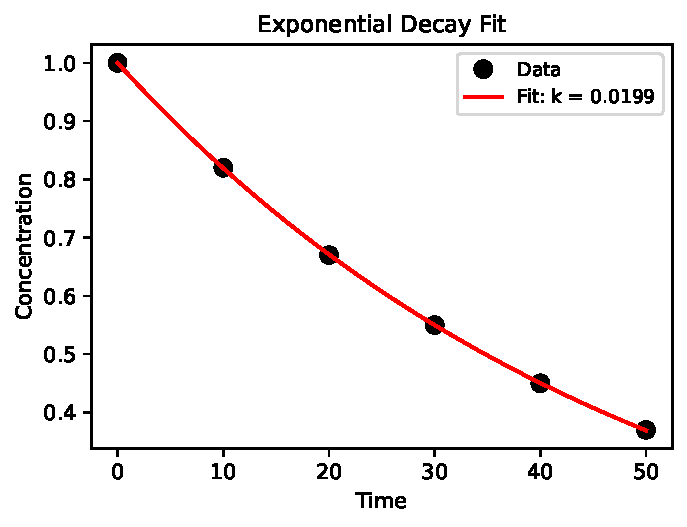
\includegraphics[width=0.7\textwidth]{figures/chap11/curve_fit_decay.pdf}
\end{center}

\begin{labexample}
Fitting a Gaussian peak to spectroscopy data:

\begin{lstlisting}
from scipy.optimize import curve_fit

def gaussian(x, amplitude, center, width, baseline):
    return amplitude * np.exp(-(x - center)**2 / (2 * width**2)) + baseline

# Simulated spectrum data
wavelengths = np.linspace(400, 600, 100)
true_peak = gaussian(wavelengths, 0.8, 500, 20, 0.1)
noise = np.random.randn(100) * 0.02
spectrum = true_peak + noise

# Fit
p0 = [0.7, 495, 25, 0.1]  # initial guesses
popt, pcov = curve_fit(gaussian, wavelengths, spectrum, p0=p0)

print(f"Peak center: {popt[1]:.1f} nm")
print(f"Peak width (sigma): {popt[2]:.1f} nm")
print(f"Peak amplitude: {popt[0]:.3f}")
\end{lstlisting}

\begin{center}
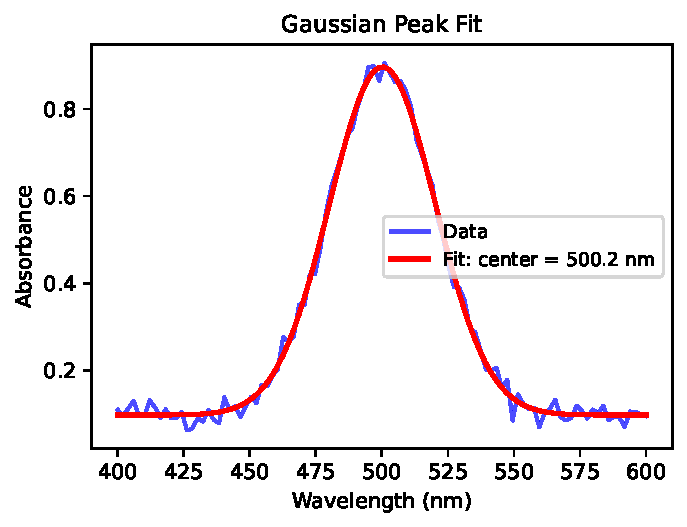
\includegraphics[width=0.7\textwidth]{figures/chap11/curve_fit_gaussian.pdf}
\end{center}
\end{labexample}

% ----------------------------------------------------------------------------
\section{Optimization}
\label{sec:optimization}

\subsection{Minimization}

\begin{lstlisting}
from scipy.optimize import minimize

# Function to minimize
def rosenbrock(x):
    return (1 - x[0])**2 + 100 * (x[1] - x[0]**2)**2

# Starting point
x0 = [0, 0]

# Minimize
result = minimize(rosenbrock, x0, method="Nelder-Mead")
print(f"Minimum at: {result.x}")
print(f"Minimum value: {result.fun}")
\end{lstlisting}

\subsection{Root Finding}

\begin{lstlisting}
from scipy.optimize import root_scalar, fsolve

# Find where f(x) = 0
def f(x):
    return x**3 - 2*x - 5

# Scalar root finding
result = root_scalar(f, bracket=[2, 3])
print(f"Root: {result.root:.6f}")

# Multiple equations
def equations(vars):
    x, y = vars
    return [x + y - 4, x * y - 3]

solution = fsolve(equations, [1, 1])
print(f"Solution: x={solution[0]:.4f}, y={solution[1]:.4f}")
\end{lstlisting}

% ----------------------------------------------------------------------------
\section{Integration}
\label{sec:integration}

\subsection{Definite Integrals}

\begin{lstlisting}
from scipy.integrate import quad

# Integrate sin(x) from 0 to pi
def f(x):
    return np.sin(x)

result, error = quad(f, 0, np.pi)
print(f"Integral: {result:.6f}")  # Should be 2.0

# With lambda
result, error = quad(lambda x: x**2, 0, 1)  # integral of x^2
\end{lstlisting}

\subsection{Differential Equations}

\begin{lstlisting}
from scipy.integrate import odeint

# First-order ODE: dy/dt = -k*y
def decay(y, t, k):
    return -k * y

k = 0.1
y0 = 1.0
t = np.linspace(0, 50, 100)

solution = odeint(decay, y0, t, args=(k,))

import matplotlib.pyplot as plt
plt.plot(t, solution)
plt.xlabel("Time")
plt.ylabel("Concentration")
\end{lstlisting}

\begin{center}
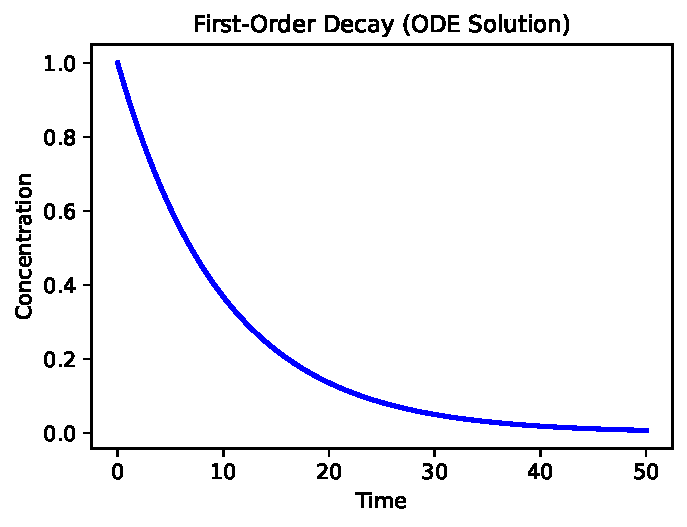
\includegraphics[width=0.7\textwidth]{figures/chap11/ode_decay.pdf}
\end{center}

\begin{labexample}
Solving coupled ODEs for a reaction A -> B -> C:

\begin{lstlisting}
from scipy.integrate import odeint

def reaction_system(y, t, k1, k2):
    A, B, C = y
    dAdt = -k1 * A
    dBdt = k1 * A - k2 * B
    dCdt = k2 * B
    return [dAdt, dBdt, dCdt]

# Parameters
k1, k2 = 0.1, 0.05
y0 = [1.0, 0.0, 0.0]  # initial: all A
t = np.linspace(0, 100, 200)

# Solve
solution = odeint(reaction_system, y0, t, args=(k1, k2))
A, B, C = solution.T

# Plot
plt.plot(t, A, label="A")
plt.plot(t, B, label="B")
plt.plot(t, C, label="C")
plt.xlabel("Time")
plt.ylabel("Concentration")
plt.legend()
\end{lstlisting}

\begin{center}
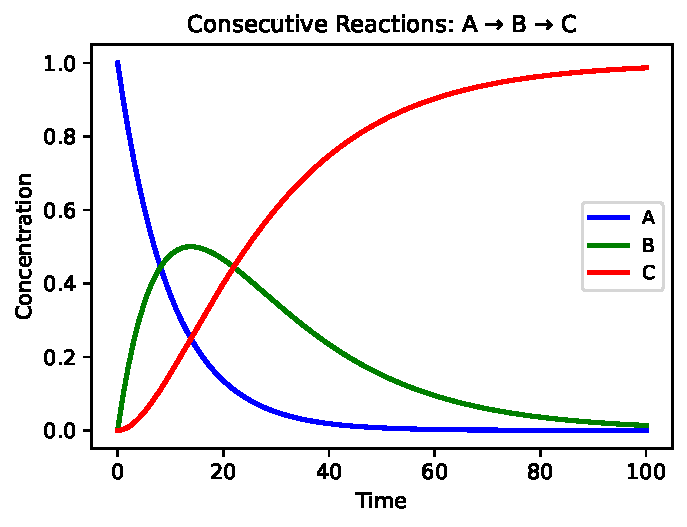
\includegraphics[width=0.7\textwidth]{figures/chap11/ode_reaction.pdf}
\end{center}
\end{labexample}

% ----------------------------------------------------------------------------
\section{Interpolation}
\label{sec:interpolation}

\begin{lstlisting}
from scipy.interpolate import interp1d

# Sparse data
x_data = np.array([0, 1, 2, 3, 4, 5])
y_data = np.array([0, 0.8, 0.9, 0.1, -0.8, -1.0])

# Create interpolation function
f_linear = interp1d(x_data, y_data, kind="linear")
f_cubic = interp1d(x_data, y_data, kind="cubic")

# Evaluate at new points
x_new = np.linspace(0, 5, 50)
y_linear = f_linear(x_new)
y_cubic = f_cubic(x_new)
\end{lstlisting}

\begin{center}
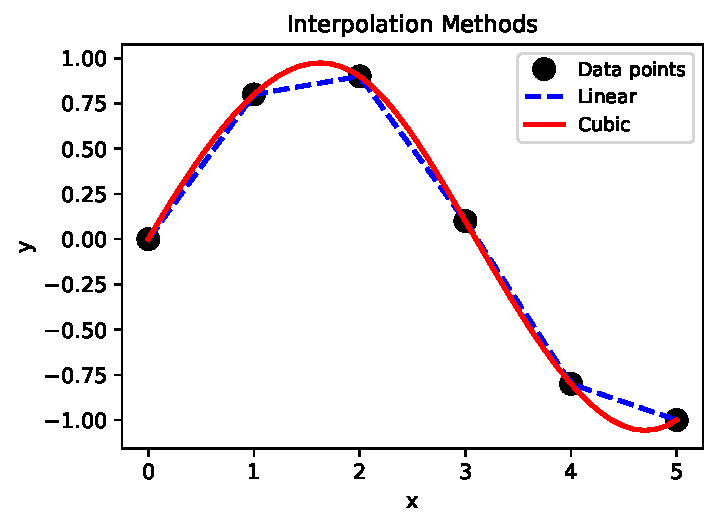
\includegraphics[width=0.7\textwidth]{figures/chap11/interpolation.pdf}
\end{center}

Interpolation types:
\begin{itemize}
    \item \py{"linear"}: straight lines between points
    \item \py{"cubic"}: smooth cubic spline
    \item \py{"nearest"}: step function
    \item \py{"quadratic"}: quadratic spline
\end{itemize}

% ----------------------------------------------------------------------------
\section{Signal Processing}
\label{sec:signal}

\subsection{Smoothing}

\begin{lstlisting}
from scipy.signal import savgol_filter
from scipy.ndimage import gaussian_filter1d

# Noisy data
x = np.linspace(0, 10, 100)
y_clean = np.sin(x)
y_noisy = y_clean + np.random.randn(100) * 0.2

# Savitzky-Golay filter
y_smooth = savgol_filter(y_noisy, window_length=11, polyorder=3)

# Gaussian smoothing
y_gauss = gaussian_filter1d(y_noisy, sigma=2)
\end{lstlisting}

\begin{center}
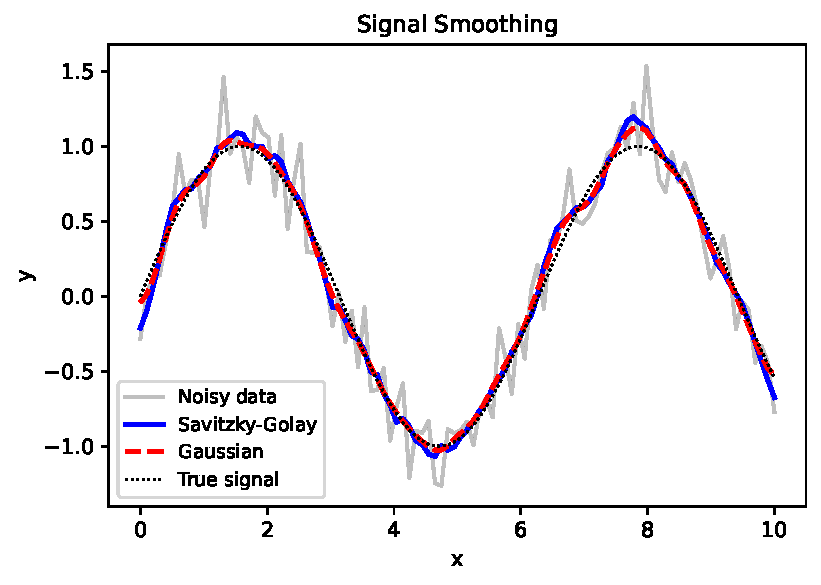
\includegraphics[width=0.7\textwidth]{figures/chap11/signal_smoothing.pdf}
\end{center}

\subsection{Peak Finding}

\begin{lstlisting}
from scipy.signal import find_peaks

# Find peaks
peaks, properties = find_peaks(y_data, height=0.5, distance=10)
print(f"Peak indices: {peaks}")
print(f"Peak heights: {properties['peak_heights']}")
\end{lstlisting}

\subsection{Fourier Transform}

\begin{lstlisting}
from scipy.fft import fft, fftfreq

# Time domain signal
dt = 0.01
t = np.arange(0, 1, dt)
signal = np.sin(2*np.pi*5*t) + 0.5*np.sin(2*np.pi*10*t)

# FFT
spectrum = fft(signal)
freqs = fftfreq(len(t), dt)

# Plot power spectrum
plt.plot(freqs[:len(freqs)//2], np.abs(spectrum[:len(spectrum)//2]))
plt.xlabel("Frequency (Hz)")
plt.ylabel("Amplitude")
\end{lstlisting}

\begin{center}
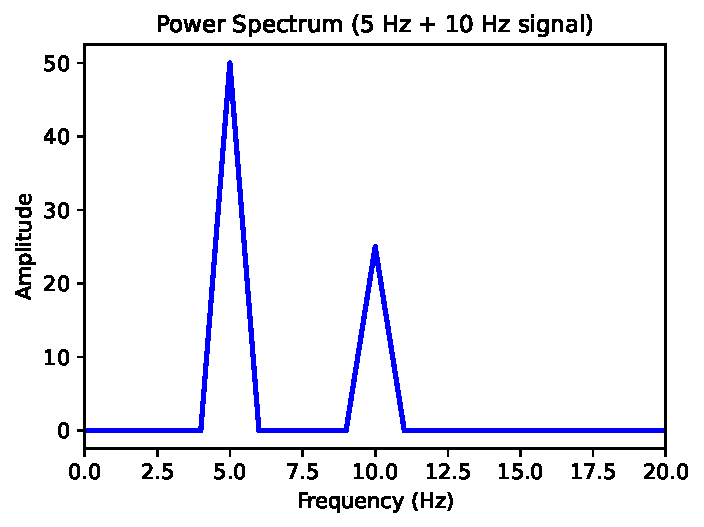
\includegraphics[width=0.7\textwidth]{figures/chap11/fft_spectrum.pdf}
\end{center}

% ----------------------------------------------------------------------------
\section{Special Functions}
\label{sec:special}

SciPy provides many mathematical special functions:

\begin{lstlisting}
from scipy import special

# Gamma function
special.gamma(5)       # 24.0 (= 4!)

# Error function
special.erf(1)         # 0.8427...

# Bessel functions
special.jv(0, 1)       # J_0(1) = 0.7652...

# Factorial
special.factorial(5)   # 120
\end{lstlisting}

% ----------------------------------------------------------------------------
\section{Physical Constants}
\label{sec:constants}

\begin{lstlisting}
from scipy import constants

constants.c           # speed of light (m/s)
constants.h           # Planck constant (J*s)
constants.k           # Boltzmann constant (J/K)
constants.R           # gas constant (J/(mol*K))
constants.N_A         # Avogadro number

# Convert units
constants.convert_temperature(100, "C", "K")  # 373.15
constants.calorie     # 1 calorie in Joules
\end{lstlisting}

% ----------------------------------------------------------------------------
\section{Chapter Summary}
\label{sec:scipy-summary}

SciPy extends NumPy with scientific algorithms:

\begin{itemize}
    \item \textbf{Statistics:} \py{stats.ttest\_ind()}, \py{stats.linregress()}, distributions
    \item \textbf{Curve fitting:} \py{optimize.curve\_fit()}
    \item \textbf{Optimization:} \py{optimize.minimize()}, \py{optimize.root\_scalar()}
    \item \textbf{Integration:} \py{integrate.quad()}, \py{integrate.odeint()}
    \item \textbf{Interpolation:} \py{interpolate.interp1d()}
    \item \textbf{Signal processing:} \py{signal.find\_peaks()}, \py{signal.savgol\_filter()}
    \item \textbf{Constants:} \py{constants.R}, \py{constants.N\_A}
\end{itemize}

\begin{ponder}
\begin{enumerate}
    \item When would you use \py{curve\_fit} vs. \py{linregress}?
    \item What's the difference between interpolation and curve fitting?
    \item How do you interpret a p-value from a t-test?
    \item Why might you need to provide initial guesses (\py{p0}) for curve fitting?
\end{enumerate}
\end{ponder}


% Part IV: Putting It Together
\part{Putting It Together}
% chap12_practical.tex - Putting it all together
% ============================================================================

\chapter{Practical Projects}
\label{chap:practical}

You've learned the pieces. Now let's put them together in complete, realistic projects. Each example demonstrates how the skills from previous chapters combine to solve actual scientific problems.

% ----------------------------------------------------------------------------
\section{Project 1: Calibration Curve Analysis}
\label{sec:project-calibration}

A common task: create a calibration curve from standards and use it to determine concentrations of unknown samples.

\begin{lstlisting}
import numpy as np
import pandas as pd
import matplotlib.pyplot as plt
from scipy.stats import linregress

# ============================================================
# Load and inspect data
# ============================================================
standards = pd.read_csv("standards.csv")
unknowns = pd.read_csv("unknowns.csv")

print("Standards:")
print(standards.head())
print("\nUnknowns:")
print(unknowns.head())

# ============================================================
# Calculate mean absorbance for each standard
# ============================================================
# Standards file has replicates
std_summary = standards.groupby("concentration")["absorbance"].agg(
    ["mean", "std", "count"]
).reset_index()
std_summary["sem"] = std_summary["std"] / np.sqrt(std_summary["count"])

# ============================================================
# Linear regression
# ============================================================
x = std_summary["concentration"].values
y = std_summary["mean"].values

result = linregress(x, y)
slope = result.slope
intercept = result.intercept
r_squared = result.rvalue ** 2

print(f"\nCalibration equation: A = {slope:.4f} * C + {intercept:.4f}")
print(f"R-squared: {r_squared:.6f}")

# ============================================================
# Create calibration plot
# ============================================================
fig, ax = plt.subplots(figsize=(8, 6))

# Plot standards with error bars
ax.errorbar(x, y, yerr=std_summary["sem"], fmt="ko",
            capsize=5, label="Standards")

# Plot regression line
x_line = np.linspace(0, x.max() * 1.1, 100)
y_line = slope * x_line + intercept
ax.plot(x_line, y_line, "r-", label=f"Fit: (*@$R^2$@*) = {r_squared:.4f}")

ax.set_xlabel("Concentration (M)")
ax.set_ylabel("Absorbance (AU)")
ax.set_title("Calibration Curve")
ax.legend()
ax.grid(True, alpha=0.3)

plt.tight_layout()
plt.savefig("calibration_curve.pdf")
\end{lstlisting}

\begin{center}
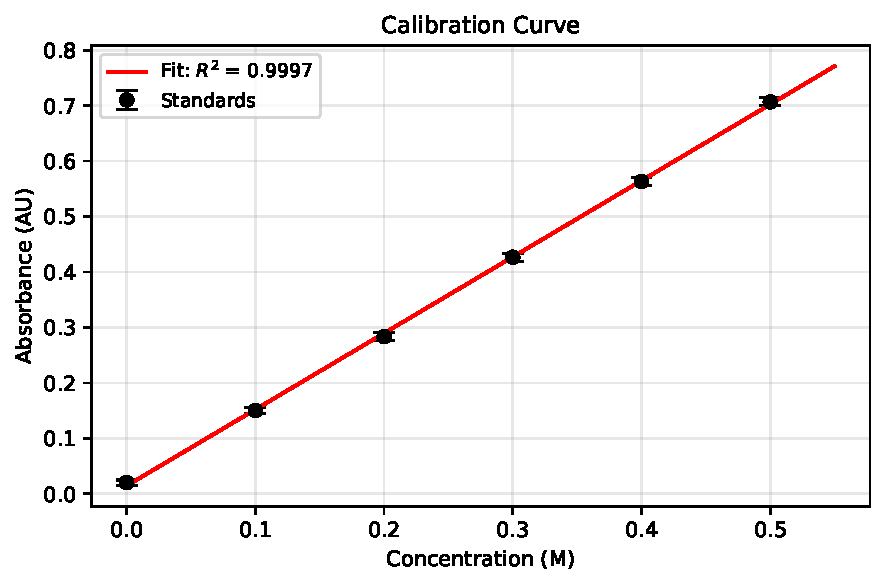
\includegraphics[width=0.75\textwidth]{figures/chap12/calibration_curve.pdf}
\end{center}

\begin{lstlisting}
# ============================================================
# Calculate unknown concentrations
# ============================================================
unknowns["concentration"] = (unknowns["absorbance"] - intercept) / slope

# Check if within calibration range
min_std = x.min()
max_std = x.max()
unknowns["in_range"] = (unknowns["concentration"] >= min_std) & \
                       (unknowns["concentration"] <= max_std)

# Flag samples outside range
outside_range = unknowns[~unknowns["in_range"]]
if len(outside_range) > 0:
    print(f"\nWarning: {len(outside_range)} samples outside calibration range")

# ============================================================
# Save results
# ============================================================
unknowns.to_csv("unknown_concentrations.csv", index=False)
print(f"\nResults saved. Processed {len(unknowns)} samples.")
\end{lstlisting}

% ----------------------------------------------------------------------------
\section{Project 2: Kinetics Data Analysis}
\label{sec:project-kinetics}

Analyze reaction kinetics data to determine rate constants and reaction order.

\begin{lstlisting}
import numpy as np
import pandas as pd
import matplotlib.pyplot as plt
from scipy.optimize import curve_fit

# ============================================================
# Load kinetics data
# ============================================================
data = pd.read_csv("kinetics_data.csv")
time = data["time_s"].values
concentration = data["concentration_M"].values

# ============================================================
# Define kinetic models
# ============================================================
def first_order(t, C0, k):
    """First-order decay: C = C0 * exp(-kt)"""
    return C0 * np.exp(-k * t)

def second_order(t, C0, k):
    """Second-order decay: 1/C = 1/C0 + kt"""
    return C0 / (1 + C0 * k * t)

# ============================================================
# Fit both models
# ============================================================
# First order
try:
    popt1, pcov1 = curve_fit(first_order, time, concentration)
    C0_1, k1 = popt1
    y_fit1 = first_order(time, *popt1)
    ss_res1 = np.sum((concentration - y_fit1)**2)
    ss_tot = np.sum((concentration - np.mean(concentration))**2)
    r2_1 = 1 - ss_res1/ss_tot
    print(f"First-order: k = {k1:.4f} (*@s$^{-1}$@*), (*@$R^2$@*) = {r2_1:.4f}")
except:
    print("First-order fit failed")

# Second order
try:
    popt2, pcov2 = curve_fit(second_order, time, concentration)
    C0_2, k2 = popt2
    y_fit2 = second_order(time, *popt2)
    ss_res2 = np.sum((concentration - y_fit2)**2)
    r2_2 = 1 - ss_res2/ss_tot
    print(f"Second-order: k = {k2:.4f} (*@M$^{-1}$s$^{-1}$@*), (*@$R^2$@*) = {r2_2:.4f}")
except:
    print("Second-order fit failed")

# ============================================================
# Determine best model
# ============================================================
if r2_1 > r2_2:
    best_model = "First-order"
    best_k = k1
    best_fit = y_fit1
else:
    best_model = "Second-order"
    best_k = k2
    best_fit = y_fit2

print(f"\nBest fit: {best_model}")

# ============================================================
# Create diagnostic plots
# ============================================================
fig, axes = plt.subplots(2, 2, figsize=(10, 8))

# Raw data with fits
ax1 = axes[0, 0]
ax1.plot(time, concentration, "ko", label="Data")
ax1.plot(time, y_fit1, "b-", label=f"1st order ((*@$R^2$@*)={r2_1:.3f})")
ax1.plot(time, y_fit2, "r--", label=f"2nd order ((*@$R^2$@*)={r2_2:.3f})")
ax1.set_xlabel("Time (s)")
ax1.set_ylabel("Concentration (M)")
ax1.legend()
ax1.set_title("Model Comparison")

# First-order linearization: ln(C) vs t
ax2 = axes[0, 1]
ax2.plot(time, np.log(concentration), "ko")
ax2.set_xlabel("Time (s)")
ax2.set_ylabel("ln(C)")
ax2.set_title("First-Order Test")

# Second-order linearization: 1/C vs t
ax3 = axes[1, 0]
ax3.plot(time, 1/concentration, "ko")
ax3.set_xlabel("Time (s)")
ax3.set_ylabel("1/C ((*@M$^{-1}$@*))")
ax3.set_title("Second-Order Test")

# Residuals for best fit
ax4 = axes[1, 1]
residuals = concentration - best_fit
ax4.plot(time, residuals, "ko")
ax4.axhline(y=0, color="r", linestyle="--")
ax4.set_xlabel("Time (s)")
ax4.set_ylabel("Residual")
ax4.set_title(f"Residuals ({best_model})")

plt.tight_layout()
plt.savefig("kinetics_analysis.pdf")
\end{lstlisting}

\begin{center}
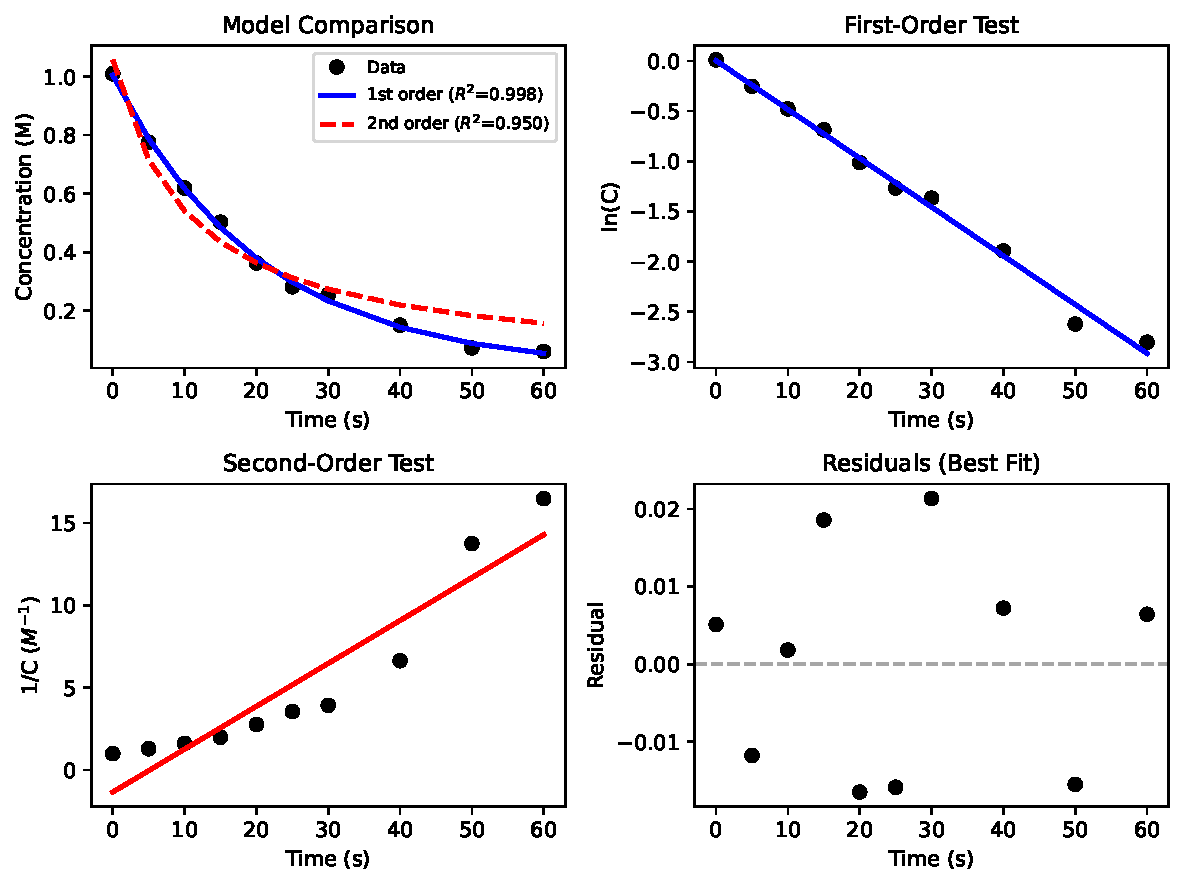
\includegraphics[width=0.85\textwidth]{figures/chap12/kinetics_analysis.pdf}
\end{center}

\begin{lstlisting}
# ============================================================
# Calculate half-life
# ============================================================
if best_model == "First-order":
    half_life = np.log(2) / best_k
else:
    half_life = 1 / (best_k * concentration[0])

print(f"Half-life: {half_life:.2f} s")
\end{lstlisting}

% ----------------------------------------------------------------------------
\section{Project 3: Batch Processing Spectra}
\label{sec:project-spectra}

Process multiple spectrum files: baseline correction, peak finding, and summary report.

\begin{lstlisting}
import numpy as np
import pandas as pd
import matplotlib.pyplot as plt
from pathlib import Path
from scipy.signal import find_peaks, savgol_filter

# ============================================================
# Setup
# ============================================================
data_folder = Path("spectra")
output_folder = Path("processed")
output_folder.mkdir(exist_ok=True)

results = []

# ============================================================
# Processing functions
# ============================================================
def load_spectrum(filepath):
    """Load spectrum from CSV file."""
    df = pd.read_csv(filepath)
    return df["wavelength"].values, df["absorbance"].values

def baseline_correct(absorbance, percentile=5):
    """Subtract baseline estimated from lowest values."""
    baseline = np.percentile(absorbance, percentile)
    return absorbance - baseline

def find_spectrum_peaks(wavelengths, absorbance, min_height=0.1):
    """Find peaks in spectrum."""
    peak_indices, properties = find_peaks(absorbance, height=min_height)
    peak_wavelengths = wavelengths[peak_indices]
    peak_heights = properties["peak_heights"]
    return list(zip(peak_wavelengths, peak_heights))

# ============================================================
# Process each file
# ============================================================
for filepath in sorted(data_folder.glob("*.csv")):
    print(f"Processing {filepath.name}...")

    # Load
    wavelengths, absorbance = load_spectrum(filepath)

    # Smooth
    abs_smooth = savgol_filter(absorbance, window_length=11, polyorder=3)

    # Baseline correct
    abs_corrected = baseline_correct(abs_smooth)

    # Find peaks
    peaks = find_spectrum_peaks(wavelengths, abs_corrected, min_height=0.05)

    # Record results
    sample_result = {
        "filename": filepath.name,
        "max_absorbance": np.max(abs_corrected),
        "num_peaks": len(peaks),
    }

    # Add first 3 peaks
    for i, (wl, height) in enumerate(peaks[:3]):
        sample_result[f"peak{i+1}_wavelength"] = wl
        sample_result[f"peak{i+1}_height"] = height

    results.append(sample_result)

    # Save processed spectrum
    processed = pd.DataFrame({
        "wavelength": wavelengths,
        "raw": absorbance,
        "smoothed": abs_smooth,
        "corrected": abs_corrected
    })
    processed.to_csv(output_folder / f"processed_{filepath.name}", index=False)

    # Create figure
    fig, ax = plt.subplots(figsize=(8, 5))
    ax.plot(wavelengths, absorbance, "gray", alpha=0.5, label="Raw")
    ax.plot(wavelengths, abs_corrected, "b-", label="Corrected")

    # Mark peaks
    for wl, height in peaks:
        ax.annotate(f"{wl:.0f}", xy=(wl, height), fontsize=8,
                   ha="center", va="bottom")

    ax.set_xlabel("Wavelength (nm)")
    ax.set_ylabel("Absorbance (AU)")
    ax.set_title(filepath.stem)
    ax.legend()

    plt.tight_layout()
    plt.savefig(output_folder / f"{filepath.stem}.png", dpi=150)
    plt.close()

# ============================================================
# Create summary
# ============================================================
summary = pd.DataFrame(results)
summary.to_csv(output_folder / "summary.csv", index=False)

print(f"\nProcessed {len(results)} files")
print(f"Results saved to {output_folder}")
print("\nSummary:")
print(summary[["filename", "max_absorbance", "num_peaks"]].to_string())
\end{lstlisting}

An example of processed output:

\begin{center}
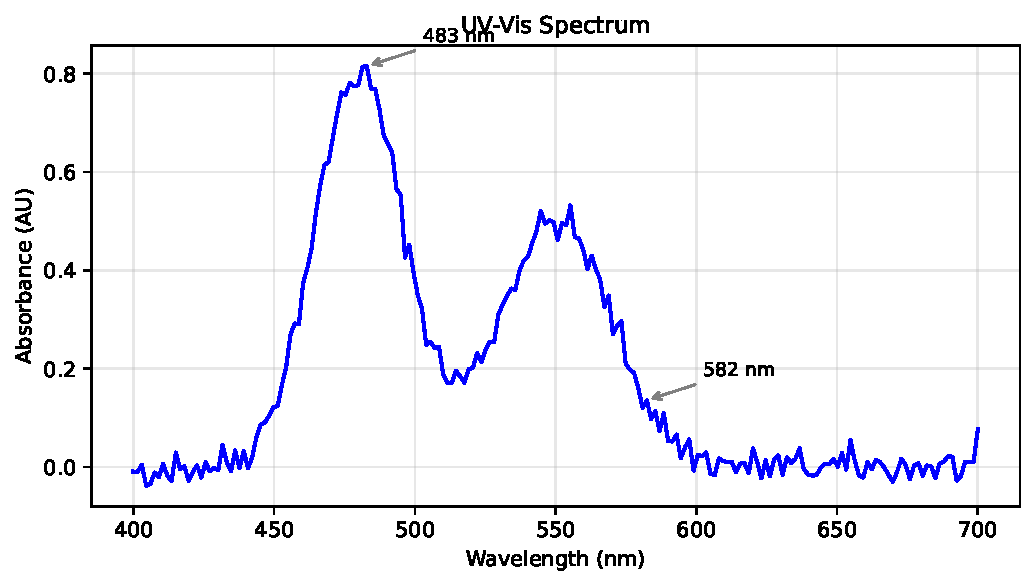
\includegraphics[width=0.75\textwidth]{figures/chap12/spectrum_example.pdf}
\end{center}

% ----------------------------------------------------------------------------
\section{Project 4: Interactive Data Dashboard}
\label{sec:project-dashboard}

Create a simple interactive analysis script with user input.

\begin{lstlisting}
import numpy as np
import pandas as pd
import matplotlib.pyplot as plt

def load_data(filepath):
    """Load data with error handling."""
    try:
        return pd.read_csv(filepath)
    except FileNotFoundError:
        print(f"Error: File '{filepath}' not found")
        return None
    except Exception as e:
        print(f"Error loading file: {e}")
        return None

def main():
    print("=" * 50)
    print("Data Analysis Dashboard")
    print("=" * 50)

    # Get filename
    filepath = input("\nEnter data file path: ").strip()
    data = load_data(filepath)

    if data is None:
        return

    print(f"\nLoaded {len(data)} rows, {len(data.columns)} columns")
    print(f"Columns: {list(data.columns)}")

    while True:
        print("\n" + "-" * 30)
        print("Options:")
        print("  1. View data summary")
        print("  2. Plot column")
        print("  3. Calculate statistics")
        print("  4. Filter data")
        print("  5. Export filtered data")
        print("  6. Exit")

        choice = input("\nSelect option (1-6): ").strip()

        if choice == "1":
            print("\nData Summary:")
            print(data.describe())

        elif choice == "2":
            print(f"\nAvailable columns: {list(data.columns)}")
            x_col = input("X column: ").strip()
            y_col = input("Y column: ").strip()

            try:
                plt.figure(figsize=(8, 6))
                plt.plot(data[x_col], data[y_col], "o-")
                plt.xlabel(x_col)
                plt.ylabel(y_col)
                plt.title(f"{y_col} vs {x_col}")
                plt.tight_layout()
                plt.show()
            except KeyError as e:
                print(f"Column not found: {e}")

        elif choice == "3":
            print(f"\nAvailable columns: {list(data.columns)}")
            col = input("Column to analyze: ").strip()

            try:
                values = data[col].dropna()
                print(f"\nStatistics for '{col}':")
                print(f"  Count: {len(values)}")
                print(f"  Mean:  {values.mean():.4f}")
                print(f"  Std:   {values.std():.4f}")
                print(f"  Min:   {values.min():.4f}")
                print(f"  Max:   {values.max():.4f}")
            except (KeyError, TypeError) as e:
                print(f"Error: {e}")

        elif choice == "4":
            print(f"\nAvailable columns: {list(data.columns)}")
            col = input("Column to filter: ").strip()
            op = input("Operator (>, <, ==): ").strip()
            val = input("Value: ").strip()

            try:
                val = float(val)
                if op == ">":
                    data = data[data[col] > val]
                elif op == "<":
                    data = data[data[col] < val]
                elif op == "==":
                    data = data[data[col] == val]
                print(f"Filtered to {len(data)} rows")
            except Exception as e:
                print(f"Error filtering: {e}")

        elif choice == "5":
            outpath = input("Output filename: ").strip()
            data.to_csv(outpath, index=False)
            print(f"Saved to {outpath}")

        elif choice == "6":
            print("Goodbye!")
            break

        else:
            print("Invalid option")

if __name__ == "__main__":
    main()
\end{lstlisting}

% ----------------------------------------------------------------------------
\section{Tips for Real Projects}
\label{sec:project-tips}

\subsection{Project Organization}

\begin{lstlisting}[style=shellstyle]
my_project/
    data/
        raw/           # original data (never modify!)
        processed/     # cleaned/processed data
    scripts/
        analyze.py
        visualize.py
        utils.py       # helper functions
    results/
        figures/
        tables/
    README.md          # project description
	main.py			   # Your main script which you run
    requirements.txt   # dependencies
\end{lstlisting}

Then, from your main script you can call functions from the scripts folder. For example, say \py{analyse.py} contains functions \py{process_data(), load_data()} and \py{visualize.py} contains \py{plot_results()} then perhaps your main script looks something like this:

\begin{lstlisting}
from scripts.analyze import load_data, process_data
from scripts.visualize import plot_results

my_data_path = "path/to/my/data.csv"
data = load_data(my_data_path)
processed_data = process_data(data)
plot_results(processed_data)
\end{lstlisting}

\subsection{Reproducibility Checklist}

\begin{itemize}
    \item Keep raw data separate and unmodified
    \item Record which script version produced each output
    \item Use \filepath{requirements.txt} to track package versions
    \item Add comments explaining non-obvious decisions
    \item Save figures as both PDF (for papers) and PNG (for presentations)
\end{itemize}

\subsection{Common Patterns}

\begin{lstlisting}
# Pattern: Process multiple files
from pathlib import Path

for filepath in Path("data").glob("*.csv"):
    data = pd.read_csv(filepath)
    result = process(data)
    result.to_csv(f"results/{filepath.stem}_processed.csv")

# Pattern: Save figure with data
fig, ax = plt.subplots()
ax.plot(x, y)
fig.savefig("plot.pdf")
pd.DataFrame({"x": x, "y": y}).to_csv("plot_data.csv")

# Pattern: Progress indicator
for i, filepath in enumerate(files):
    print(f"Processing {i+1}/{len(files)}: {filepath.name}")
    # process file
\end{lstlisting}

\begin{tip}
If progress bars end up being important to your project, check out the package \py{tqdm} for polished progress bars with duration estimates built in.
\end{tip}

\begin{ponder}
\begin{enumerate}
    \item What repetitive tasks in your research could Python automate?
    \item How would you modify the calibration project to handle non-linear calibration curves?
    \item Design a project to analyze data from your own research.
    \item What error handling would you add to make these scripts more robust?
\end{enumerate}
\end{ponder}


\part{Closing Remarks}
% closing_remarks.tex - Final chapter closing and resources
% ============================================================================

\section{Where to Go From Here}
\label{sec:next-steps}

This book gave you the essentials. The real learning happens when you start using Python for your own research. Here are resources to help you continue.

\subsection{Packages to Explore}

These libraries extend your toolkit for specific tasks. With what you've learned, you can teach yourself any of them from their documentation:

\begin{itemize}
    \item \textbf{seaborn} --- Statistical visualization built on Matplotlib. Less code, beautiful plots.
    \item \textbf{scikit-learn} --- Machine learning.
    \item \textbf{statsmodels} --- Statistical modeling: linear models, time series, hypothesis tests.
    \item \textbf{sympy} --- Symbolic mathematics: algebra, calculus, equation solving (Mathematica like).
    \item \textbf{lmfit} --- Curve fitting with parameter constraints, confidence intervals, \& model evaluation.
    \item \textbf{uncertainties} --- Automatic error propagation through calculations.
    \item \textbf{pint} --- Physical units handling (never confuse meters and feet again).
\end{itemize}

\subsection{Domain-Specific Libraries}

Search for Python packages in your field---they almost certainly exist:
\begin{itemize}
    \item \textbf{Chemistry:} RDKit, Open Babel, cclib, PyMOL
    \item \textbf{Biology:} Biopython, scikit-bio, scanpy
    \item \textbf{Physics/Astronomy:} Astropy, QuTiP, PyMC
    \item \textbf{Geoscience:} xarray, cartopy, MetPy
    \item \textbf{Image Analysis:} scikit-image, OpenCV, Pillow
\end{itemize}

\subsection{Improve Your Workflow}

As your projects grow, these practices will save you time and headaches:
\begin{itemize}
    \item Learn Git for version control
    \item Write tests for your code
    \item Create reusable packages from your scripts
    \item Explore Jupyter notebooks for interactive analysis
\end{itemize}



\subsection{Practice}

The best way to learn is to use Python for something you actually care about. Pick a dataset from your research. Automate something tedious. Recreate a figure from a paper. Break things, fix them, and learn by doing.

You now have enough foundation to teach yourself the rest.

\subsection{Where to Get Help}
If you do get stuck (and you will be---everyone does) in order of quality:
\begin{itemize}
    \item \textbf{Official Documentation} --- NumPy, Pandas, and Matplotlib all have excellent tutorials and example galleries.
	\item \textbf{Your colleagues}---They will often know more about the specific problems you're trying to solve than most others.
    \item \textbf{Stack Overflow} --- Search before asking. Your error message has almost certainly been answered.
    \item \textbf{GitHub Issues} --- For package-specific bugs or feature questions.
    \item \textbf{Reddit} --- r/learnpython is friendly to beginners; r/Python for general discussion.
	\item \textbf{Chat-bots}---Undeniably useful, even if these can be problematic. Use with caution, and don't accept code you don't understand. These are a double-edged blade, you WILL get cut using these.
\end{itemize}

\begin{warning}
While AI chatbots can be helpful, they are a double-edged sword for beginners. To get a functional result, you often have to describe your problem in such extreme detail that you might as well have written the code yourself. In fact, Python is likely the most efficient language for that description, so with the description done, you have what you wanted. 

Anything less than a perfect prompt usually results in "black box" code: bloated, difficult to debug, and hard to learn from. However, they can be excellent tools if used as a \textbf{reference} rather than a \textbf{ghostwriter}. Chat-bots give you speed, and so if you're bad at the task, now you're just bad faster. Do not mistake speed for efficiency or effectiveness.

\textbf{Chatbots may be effective for:}
\begin{itemize}
    \item \textbf{Search:} ``Is there a NumPy function that calculates the standard deviation?''
    \item \textbf{Syntax:} ``How do I format a f-string to show two decimal places?''
    \item \textbf{Error Decoding:} Pasting an error message to get a plain-English explanation of what it means. \textbf{AFTER} you have tried to understand yourself a few times. Do not default to a bot when running into problems, it robs you of skills and experiences that are worth more than whatever deadline feels important right now.
\end{itemize}

\textbf{Avoid Chatbots for:}
\begin{itemize}
    \item \textbf{Logic:} Asking it to write a whole script. You lose the "mental muscle" built by solving the puzzle yourself. Besides, given what you do, you are quite likely better at logic than a chat-bot.
    \item \textbf{Debugging:} Letting it guess fixes for your code. You will often spend more time trying to fix the chatbot's "fix" than if you had used \texttt{print()} statements to find the bug yourself.
\end{itemize}
\end{warning}

\vfill
\begin{center}
    \textit{Happy Coding!}
\end{center}

% ----------------------------------------------------------------------------
% BACK MATTER
% ----------------------------------------------------------------------------
\backmatter

% Future additions
% \input{backmatter/appendix_install}
% \input{backmatter/appendix_troubleshooting}
% \input{backmatter/bibliography}
% \input{backmatter/index}

\end{document}
